\documentclass[letterpaper,11pt,leqno]{book}
\usepackage{float}
\usepackage{longtable}
\usepackage{book}

\usepackage[utf8]{inputenc}
\usepackage[vietnamese]{babel}
\usepackage{graphicx}
\usepackage{float}

\usepackage{graphicx}
\usepackage{float}
\usepackage[utf8]{inputenc}
\usepackage{float}
\usepackage[vietnamese]{babel}

% Bổ sung các package cần thiết
\usepackage{microtype} 
\usepackage{hyperref} 
\usepackage{longtable}
\usepackage{amsmath}

% Disable font expansion for bitmap Vietnamese fonts used by pdfTeX.
\microtypesetup{expansion=false}
\bibliographystyle{book}

% Enter book title to populate PDF metadata:
\hypersetup{pdftitle={Thiết Kế Cơ Sở Dữ Liệu - LivingDocs}}

% Enter path to BibTeX file with references:
\newcommand{\bib}{book.bib}

% Enter path to PDF file with figures:
\newcommand{\pdf}{figures.pdf}

\begin{document}

% Enter title:

\title{Thiết Kế Cơ Sở Dữ Liệu}

\title{Research Monograph}


% Enter subtitle (can be commented out):
\subtitle{Đề Tài: LivingDocs}

% Enter author:
\author{Nhóm 1}

% Enter date:
\date{2026}

\begin{titlepage}
\maketitle
\end{titlepage}

\frontmatter

\tableofcontents

% Enter book structure
\chapter{Giới Thiệu Đề Tài}

\section*{Tổng quan đề tài}
Trong quy trình phát triển phần mềm hiện đại, việc duy trì tính nhất quán giữa tài liệu kỹ thuật (\textit{Documentation}) và mã nguồn thực tế (\textit{Git Codebase}) là một thách thức lớn. Hiện tượng \textbf{"Trôi lệch tài liệu"} (\textit{Documentation Drift}) thường xuyên xảy ra khi mã nguồn liên tục được cập nhật nhưng tài liệu không được điều chỉnh kịp thời, dẫn đến lãng phí thời gian bảo trì và gia tăng rủi ro trong vận hành hệ thống.

Hệ thống \textbf{LivingDocs} ra đời như một giải pháp toàn diện giúp tự động hóa việc đồng bộ, kiểm duyệt và quản lý tài liệu kỹ thuật theo vết mã nguồn. Hệ thống tích hợp công nghệ AI (\textit{AI Grounding}) để đối soát minh chứng trực tiếp giữa các đoạn mã nguồn với văn bản tài liệu, phát hiện và cảnh báo kịp thời sự trôi lệch dữ liệu.

\section*{Phạm vi Kiến trúc Cơ sở Dữ liệu}
Nhóm thực hiện đề tài xây dựng và thiết kế kiến trúc Cơ sở dữ liệu (CSDL) cho hệ thống \textbf{LivingDocs}, bao phủ 5 phân hệ nghiệp vụ nòng cốt:

\begin{itemize}
    \item \textbf{Phân hệ Quản trị \& Phân quyền (\textit{Auth \& Workspace Domain}):} Quản lý thông tin người dùng (\texttt{users}), tổ chức không gian làm việc (\texttt{workspaces}), cấu trúc vai trò (\texttt{roles}) và chi tiết quyền hạn (\texttt{permissions}).
    \item \textbf{Phân hệ Tích hợp Mã nguồn (\textit{Git Repository Domain}):} Đồng bộ cấu trúc dữ liệu từ Git bao gồm kho mã nguồn (\texttt{repositories}), nhánh (\texttt{branches}), lịch sử thay đổi (\texttt{commits}), yêu cầu hợp nhất (\texttt{pull\_requests}) và các thực thể mã nguồn thu được từ cây AST (\texttt{code\_entities}).
    \item \textbf{Phân hệ Tài liệu \& AI Minh chứng (\textit{Documentation \& AI Domain}):} Quản lý dàn ý mẫu (\texttt{templates}), các mục dàn ý (\texttt{template\_sections}), biến chèn (\texttt{placeholders}), tài liệu (\texttt{documents}), các phiên bản tài liệu (\texttt{document\_versions}), dữ liệu đối soát AI (\texttt{grounding\_evidences}) và hệ thống cảnh báo trôi lệch (\texttt{drift\_alerts}).
    \item \textbf{Phân hệ Kiểm duyệt Kỹ thuật (\textit{Code Review Domain}):} Quản lý các phiên review tài liệu (\texttt{reviews}), các quyết định phê duyệt (\texttt{approvals}) và luồng bình luận góp ý (\texttt{review\_comments}).
    \item \textbf{Phân hệ Cấu hình \& Nhật ký (\textit{Preferences \& Audit Logs}):} Quản lý cấu hình thông báo cá nhân (\texttt{user\_notification\_preferences}), tích hợp kết nối GitHub (\texttt{github\_connections}) và lưu trữ nhật ký biến động hệ thống (\texttt{change\_logs}).
\end{itemize}

\section*{Phương pháp Nghiên cứu và Quy trình Triển khai CSDL}
Để đảm bảo CSDL của hệ thống LivingDocs đạt tính toàn vẹn, tối ưu hiệu năng và triệt tiêu dư thừa dữ liệu, đồ án áp dụng quy trình thiết kế CSDL chuẩn mực qua 3 mức biểu diễn kết hợp triển khai các thuật toán nền tảng của môn học Thiết kế Cơ sở Dữ liệu:

\begin{center}
\begin{small}
\begin{verbatim}
                 Đặc tả Yêu cầu Nghiệp vụ
                            |
                            |  (Áp dụng Thuật toán 2.1)
                            v
           Mức Quan niệm (Conceptual ERD / UML)
                            |
                            |  (Áp dụng Thuật toán 2.2 & 2.3)
                            v
         Mức Lô-gíc (Logical Relational Schema)
                            |
                            |  (Phân tích FDs & Chứng minh 3NF)
                            v
            Mức Vật lý (Physical DDL Scripts)
\end{verbatim}
\end{small}
\end{center}


\mainmatter

\part{Thiết Kế Quan Niệm }\label{p:first}

\chapter{Thuật toán 2.1  \& Mô hình Conceptual ERD}\label{c:task_1}

% Include the chapter only when its source file is present.
% This prevents compilation from stopping if chapter1.tex is not available.




Ở mức thiết kế quan niệm (\textit{Conceptual Design Level}), mục tiêu cốt lõi là chuyển hóa các mô tả nghiệp vụ thô, yêu cầu chức năng và quy tắc hệ thống thành mô hình dữ liệu trừu tượng, hoàn toàn độc lập với Hệ quản trị cơ sở dữ liệu (DBMS). Đồ án áp dụng \textbf{Thuật toán 2.1} (\textit{Algorithm 2.1: Thiết kế Sơ đồ ER từ Yêu cầu Nghiệp vụ}) để đảm bảo tính toàn vẹn và phản ánh chính xác các nghiệp vụ cốt lõi của hệ thống \textbf{LivingDocs — Design and Implementation of an AI-Assisted Self-Updating Document System for Engineering Teams}.

Quá trình này tiếp nhận đầu vào (\textit{Input}) là bài toán giải quyết hiện tượng trôi lệch tài liệu (\textit{Documentation Drift}), bộ yêu cầu chức năng từ 5 vai trò người dùng (\textit{Developer, Staff, Manager, Technical Lead, Administrator}) và kết xuất đầu ra (\textit{Output}) là Sơ đồ Quan niệm (\textit{Conceptual ERD/UML}) đã qua kiểm chứng.





\section{Phân loại Tác nhân \& Phạm vi Nghiệp vụ }
\label{sec:actor-classification}
\begingroup
\setlength{\tabcolsep}{4pt} % Khoảng đệm giữa các cột
\small % Dùng cỡ chữ \small giúp nội dung lấp đầy bảng đẹp mắt hơn

\begin{longtable}{|
>{\raggedright\arraybackslash}p{0.13\textwidth}|
>{\raggedright\arraybackslash}p{0.17\textwidth}|
>{\raggedright\arraybackslash}p{0.35\textwidth}|
>{\raggedright\arraybackslash}p{0.13\textwidth}|
>{\raggedright\arraybackslash}p{0.13\textwidth}|}
\hline

\textbf{Tác nhân} &
\textbf{Mục tiêu} &
\textbf{Nhiệm vụ \& Quyền hạn chính} &
\textbf{Phạm vi dữ liệu} &
\textbf{Đặc điểm cốt lõi} \\
\hline
\endhead % Lặp lại dòng tiêu đề khi bảng ngắt sang trang sau

\textbf{Developer} &
Khởi tạo và sử dụng tài liệu phần mềm. &
Kết nối GitHub và chọn Repository vào Workspace; yêu cầu AI sinh tài liệu theo Template; xem Grounding Evidence; chỉnh sửa bản nháp và Submit; bật/tắt Auto-update; xem Version History và Drift Alert. &
Workspace và Repository được cấp quyền; không có quyền Approve hoặc Publish. &
Là tác nhân \textbf{duy nhất khởi tạo} vòng đời tài liệu, bắt đầu luồng \textbf{AI $\rightarrow$ Staff $\rightarrow$  Manangerr}. \\
\hline

\textbf{Staff} &
Thực hiện review kỹ thuật cấp 1. &
Xem Review Queue; kiểm tra Grounding Evidence, Source File, Code Entity, Commit, Code Diff và Change Log; kiểm tra Template; Comment, sửa lỗi nhỏ; Approve hoặc Reject và trả về Developer. &
Toàn bộ bối cảnh kỹ thuật của tài liệu đang review; không có quyền Publish hoặc Commit. &
Là \textbf{cổng lọc kỹ thuật}, phát hiện sai sót và AI hallucination trước khi chuyển đến Manager. \\
\hline

\textbf{Manager} &
Phê duyệt cuối và quyết định xuất bản tài liệu. &
Xem kết quả Staff review, Comment và Grounding Evidence; thực hiện Approve, Reject hoặc Rollback; quản lý danh mục tài liệu cần Manager approval; xem lịch sử Approval. &
Tài liệu đã qua Staff review và thuộc phạm vi quản lý. &
Là tác nhân \textbf{duy nhất} có quyền Publish hoặc Commit tài liệu vào Repository thật. \\
\hline

\textbf{Technical Lead} &
Quản trị chất lượng và chính sách tài liệu. &
Quản lý Documentation Collection và Ownership; thiết lập chính sách và ngưỡng phát hiện tài liệu lỗi thời ; quản lý Template, Section, Heading, Placeholder và ánh xạ Placeholder $\leftrightarrow$ Code Entity. &
Toàn bộ Workspace và Repository thuộc phạm vi quản lý. &
Tập trung vào \textbf{Policy, Threshold và Template}, không review từng tài liệu như Manager. \\
\hline

\textbf{Admin} &
Vận hành hạ tầng và quản trị hệ thống. &
Quản lý Tài khoản \& Phân quyền:  User, Role, Permission, Workspace và Repository và cấu hình tích hợp \& hạ tầng như GitHub App, OAuth, GitHub Actions, tích hợp GitLab, Jira, Slack; cấu hình ngôn ngữ và AI Model. &
Toàn bộ hệ thống ở cấp độ hạ tầng và kỹ thuật; không review hoặc approve tài liệu. &
Là tác nhân \textbf{duy nhất} quản lý cấu hình AI Model như LLM và Embedding, nằm ngoài luồng phê duyệt tài liệu. \\
\hline

\end{longtable}
\endgroup
\section{Chi tiết các Thực thể Dữ liệu Cốt lõi (Core Data Entities)}


\section{Chi tiết các Thực thể Dữ liệu}

% LaTeX does not define a fourth-level sectioning command by default.
\providecommand{\subsubsubsection}[1]{\paragraph{#1}}

\subsection{Nhóm Quản trị \& Kết nối}

\subsubsection{User (Thực thể mạnh)}

Người dùng cuối trong hệ thống (Developer, Staff, Manager, Tech Lead, Admin).

\subsubsubsection{Thuộc tính Phức hợp (Composite Attribute)}

\begin{itemize}
    \item \textbf{FullName:} Thuộc tính phức hợp gồm:
    \begin{itemize}
        \item FirstName
        \item LastName
    \end{itemize}
\end{itemize}

\subsubsubsection{Thuộc tính Đa trị (Multi-valued Attribute)}

\begin{itemize}
    \item \textbf{NotificationPreferences (Cài đặt thông báo):}
    Lưu nhiều giá trị cùng lúc cho một người dùng
    (ví dụ: chọn đồng thời cả \texttt{EMAIL} và \texttt{SYSTEM}).
\end{itemize}

\subsubsubsection{Thuộc tính Đơn (Simple / Atomic Attribute)}

\begin{itemize}
    \item \textbf{user\_id (PK):UUID} Định danh duy nhất cho từng người dùng.
    \item \textbf{email:} Địa chỉ email bắt buộc dùng để đăng nhập và nhận thông báo hệ thống.
    \item \textbf{password\_hash:} Mật khẩu đã mã hóa. Lưu giá trị khi đăng nhập bằng Email/Password và giữ \textbf{NULL} khi dùng thuần GitHub OAuth.
    \item \textbf{status:} Trạng thái tài khoản (ACTIVE, INACTIVE, BLOCKED).
    \item \textbf{created\_at:} Thời điểm khởi tạo tài khoản.
    \item \textbf{updated\_at:} Thời điểm cập nhật thông tin gần nhất.
    \item \textbf{deleted\_at:} Soft delete nhằm giữ nguyên lịch sử giao dịch (review, comment, approval) khi người dùng rời hệ thống.
\end{itemize}


\subsection{Workspace (Thực thể mạnh)}

Không gian làm việc chứa repository và tài liệu của một nhóm/dự án.

\subsubsection{Thuộc tính Đơn (Simple / Atomic Attribute)}

\begin{itemize}
    \item \textbf{workspace\_id (PK):UUID} Định danh duy nhất cho từng không gian làm việc.
    \item \textbf{name:} Tên không gian làm việc/dự án (VD: ``Payment Service Platform'').
    \item \textbf{description:} Mô tả chi tiết về phạm vi và mục tiêu của workspace.
    \item \textbf{status:} Trạng thái hoạt động của workspace (ACTIVE, ARCHIVED).
    \item \textbf{created\_at:} Thời điểm khởi tạo workspace.
    \item \textbf{updated\_at:} Thời điểm cập nhật thông tin workspace gần nhất.
    \item \textbf{deleted\_at:} Cờ xóa mềm (Soft delete) giữ nguyên dữ liệu báo cáo và audit trail khi ẩn workspace.
\end{itemize}


\subsection{Role (Thực thể mạnh)}

Vai trò của người dùng, được scoped theo Workspace.

\subsubsection{Thuộc tính Đơn (Simple / Atomic Attribute)}

\begin{itemize}
    \item \textbf{role\_id (PK):UUID} Định danh duy nhất cho vai trò.
    \item \textbf{role\_name:} Tên vai trò (VD: Developer, Staff, Manager, Tech Lead, Admin).
    \item \textbf{description:} Mô tả tóm tắt mục đích và quyền hạn chung của vai trò.
    \item \textbf{created\_at:} Thời điểm khởi tạo vai trò trong hệ thống.
    \item \textbf{updated\_at:} Thời điểm cập nhật vai trò gần nhất.
\end{itemize}


\subsubsection{Permission (Thực thể mạnh)}

Quyền hạn chi tiết trên hệ thống (VD: DOC\_APPROVE, TEMPLATE\_EDIT).

\subsubsubsection{Thuộc tính Đơn (Atomic Attribute)}

\begin{itemize}
    \item \textbf{permission\_id (PK):UUID} Định danh duy nhất cho quyền.
    \item \textbf{permission\_code:} Mã quyền thao tác hệ thống (VD: DOC\_APPROVE, TEMPLATE\_EDIT).
    \item \textbf{description:} Giải thích chi tiết giới hạn của thao tác này.
    \item \textbf{created\_at:} Mốc thời gian quyền được khởi tạo vào danh mục hệ thống.
\end{itemize}


\subsubsection{RolePermission (Thực thể liên kết)}

Bản ghi phân quyền chi tiết cho từng vai trò trong hệ thống.

\subsubsubsection{Thuộc tính Đơn (Atomic Attribute)}

\begin{itemize}
    \item \textbf{role\_permission\_id (PK):UUID} Định danh duy nhất cho bản ghi phân quyền (UUID).
    \item \textbf{role\_id (FK):UUID} Khóa ngoại trỏ đến vai trò được gán quyền (roles).
    \item \textbf{permission\_id (FK):UUID} Khóa ngoại trỏ đến quyền hạn cụ thể (permissions).
    \item \textbf{created\_at:} Mốc thời gian quyền này được gán cho vai trò.
\end{itemize}


\subsubsection{WorkspaceMember (Thực thể mối kết hợp)}

Ghi nhận sự tham gia của User trong Workspace và vai trò (Role) tương ứng.

\subsubsubsection{Thuộc tính Đơn (Atomic Attribute)}

\begin{itemize}
    \item \textbf{member\_id (PK):UUID} Định danh duy nhất cho bản ghi tham gia.
    \item \textbf{status:} Trạng thái thành viên (ACTIVE, INACTIVE, REMOVED).
    \item \textbf{joined\_at:} Thời điểm người dùng chính thức tham gia.
    \item \textbf{created\_at:} Thời điểm gửi lời mời / tạo bản ghi.
    \item \textbf{updated\_at:} Thời điểm cập nhật vai trò hoặc trạng thái gần nhất.
\end{itemize}


\subsubsection{GitHubConnection (Thực thể phụ thuộc)}

Lưu thông tin xác thực OAuth của User với GitHub.

\paragraph{Thuộc tính Khóa (Key Attribute)}

\begin{itemize}
    \item \textbf{connection\_id:} Định danh duy nhất cho bản ghi kết nối OAuth.
\end{itemize}

\paragraph{Thuộc tính Đơn / Nguyên tố (Simple / Atomic Attributes)}

\begin{itemize}
    \item \textbf{github\_user\_id:} ID tài khoản người dùng trên hệ thống GitHub để đối soát định danh.
    \item \textbf{github\_username:} Tên tài khoản GitHub (VD: octocat).
    \item \textbf{access\_token:} Chuỗi token ủy quyền dùng để gọi GitHub API.
    \item \textbf{created\_at:} Thời điểm người dùng thực hiện liên kết tài khoản.
    \item \textbf{updated\_at:} Thời điểm làm mới token hoặc cập nhật quyền hạn gần nhất.
\end{itemize}

\subsubsubsection{Thuộc tính Đa trị (Multi-valued Attribute)}

\begin{itemize}
    \item \textbf{scopes:} Lưu danh sách các phạm vi quyền OAuth được cấp phép cùng lúc (VD: repo, read:user, workflow).
\end{itemize}


\subsection{Nhóm Mã nguồn \& Cấu trúc Code}

\subsubsection{Repository (Thực thể mạnh)}

Kho chứa mã nguồn được đồng bộ vào hệ thống.

\subsubsubsection{Thuộc tính Đơn (Atomic Attribute)}

\begin{itemize}
    \item \textbf{repository\_id (PK):UUID} Định danh duy nhất cho kho mã nguồn.
    \item \textbf{name:} Tên kho mã nguồn (VD: payment-gateway).
    \item \textbf{url:} Đường dẫn gốc đến kho chứa trên VCS.
    \item \textbf{default\_branch:} Nhánh mặc định dùng để phân tích code (VD: main, master).
    \item \textbf{sync\_status:} Trạng thái đồng bộ dữ liệu (SYNCING, SUCCESS, FAILED).
    \item \textbf{last\_synced\_at:} Thời điểm đồng bộ mã nguồn thành công gần nhất.
    \item \textbf{created\_at:} Thời điểm tích hợp kho mã nguồn vào hệ thống.
    \item \textbf{updated\_at:} Thời điểm cập nhật trạng thái hoặc cấu hình kho gần nhất.
\end{itemize}


\subsubsection{Branch (Thực thể yếu -- phụ thuộc Repository)}

Nhánh phát triển trong repository.

\subsubsubsection{Thuộc tính Đơn (Simple / Atomic Attribute)}

\begin{itemize}
    \item \textbf{branch\_id (PK):UUID} Định danh duy nhất cho nhánh.
    \item \textbf{branch\_name:} Tên nhánh (VD: main, staging, feature/auth).
    \item \textbf{is\_default:} Cờ xác định nhánh mặc định của repo (true/false).
    \item \textbf{created\_at:} Thời điểm nhánh được nhận diện và lưu vào hệ thống.
    \item \textbf{updated\_at:} Thời điểm cập nhật commit hash hoặc trạng thái nhánh gần nhất.
\end{itemize}


\subsubsection{Commit (Thực thể yếu -- phụ thuộc Branch/Repository)}

Bản ghi một lần commit mã nguồn.

\subsubsubsection{Thuộc tính Phức hợp (Composite Attribute)}

\begin{itemize}
    \item \textbf{AuthorInfo:} Thông tin tác giả thực hiện commit, gồm:
    \begin{itemize}
        \item AuthorName
        \item AuthorEmail
    \end{itemize}
\end{itemize}

\subsubsubsection{Thuộc tính Đơn (Simple / Atomic Attribute)}

\begin{itemize}
    \item \textbf{commit\_id (PK):UUID} Định danh nội bộ cho bản ghi commit.
    \item \textbf{commit\_hash:} Mã băm SHA-1/SHA-256 duy nhất từ Git (VD: 7a8f9b2...).
    \item \textbf{message:} Nội dung mô tả của commit.
    \item \textbf{committed\_at:} Thời điểm commit được thực hiện trên VCS (thời gian nghiệp vụ).
    \item \textbf{created\_at:} Thời điểm bản ghi commit được đồng bộ vào LivingDocs (thời gian hệ thống).
\end{itemize}


\subsubsection{PullRequest (Thực thể yếu -- phụ thuộc Repository)}

Yêu cầu hợp nhất nhánh từ GitHub.

\subsubsubsection{Thuộc tính Đa trị (Multi-valued Attribute)}

\begin{itemize}
    \item \textbf{labels:} Danh sách nhãn phân loại được gắn trên PR
    (VD: bug, enhancement, documentation, api-change).
\end{itemize}

\subsubsubsection{Thuộc tính Đơn (Simple / Atomic Attribute)}

\begin{itemize}
    \item \textbf{pr\_id (PK):UUID} Định danh nội bộ của bản ghi PR.
    \item \textbf{pr\_number:} Số thứ tự PR trên nền tảng gốc (VD: \#102, \#123).
    \item \textbf{title:} Tiêu đề của Pull Request.
    \item \textbf{description:} Nội dung văn bản mô tả chi tiết PR, là dữ liệu đầu vào cho AI.
    \item \textbf{source\_branch:} Nhánh nguồn chứa mã nguồn thay đổi.
    \item \textbf{target\_branch:} Nhánh đích dự định hợp nhất vào (VD: main, develop).
    \item \textbf{status:} Trạng thái vòng đời của PR (OPEN, MERGED, CLOSED).
    \item \textbf{created\_at:} Thời điểm mở PR trên VCS.
    \item \textbf{updated\_at:} Thời điểm PR cập nhật thông tin/trạng thái gần nhất.
    \item \textbf{merged\_at:} Thời điểm PR chính thức được chấp nhận hợp nhất (Nullable).
\end{itemize}


\subsubsection{CodeDiff (Thực thể yếu -- phụ thuộc Commit/PR)}

Chi tiết thay đổi mã nguồn trong commit hoặc PR.

\subsubsubsection{Thuộc tính Đơn (Simple / Atomic Attribute)}

\begin{itemize}
    \item \textbf{diff\_id (PK):UUID} Định danh nội bộ bản ghi chi tiết thay đổi.
    \item \textbf{file\_path:} Đường dẫn tương đối đến tệp bị thay đổi (VD: src/controllers/payment.js).
    \item \textbf{change\_type:} Loại thao tác trên file (ADD, MODIFY, DELETE, RENAME).
    \item \textbf{additions:} Số dòng code được thêm mới.
    \item \textbf{deletions:} Số dòng code bị xóa đi.
    \item \textbf{diff\_content:} Nội dung chi tiết các đoạn code thay đổi (patch/hunk text) dùng làm input cho AI.
    \item \textbf{created\_at:} Thời điểm lưu bản ghi diff vào hệ thống.
\end{itemize}


\subsubsection{File (Thực thể yếu -- phụ thuộc Repository)}

Cấu trúc tập tin mã nguồn trong kho chứa.

\subsubsubsection{Thuộc tính Đơn (Simple / Atomic Attribute)}

\begin{itemize}
    \item \textbf{file\_id (PK):UUID} Định danh nội bộ của tập tin trong hệ thống.
    \item \textbf{file\_path:} Đường dẫn đầy đủ của file tính từ gốc repository.
    \item \textbf{file\_type:} Loại hoặc đuôi mở rộng của tệp (VD: ts, java, py, md).
    \item \textbf{status:} Trạng thái của file trong cây thư mục (ACTIVE, DELETED, RENAMED).
    \item \textbf{created\_at:} Thời điểm file lần đầu được ghi nhận vào hệ thống.
    \item \textbf{updated\_at:} Thời điểm thông tin file hoặc nội dung file thay đổi gần nhất.
\end{itemize}


\subsubsection{CodeEntity (Thực thể yếu -- phụ thuộc File)}

Đơn vị mã nguồn cụ thể thu được từ AST (Class, Method, Function...).

\subsubsubsection{Thuộc tính Phức hợp (Composite Attribute)}

\begin{itemize}
    \item \textbf{position:} Vị trí của thực thể trong tập tin, gồm:
    \begin{itemize}
        \item \textbf{start\_line:} Dòng bắt đầu của thực thể code.
        \item \textbf{end\_line:} Dòng kết thúc của thực thể code.
    \end{itemize}
\end{itemize}

\subsubsubsection{Thuộc tính Đơn (Simple / Atomic Attribute)}

\begin{itemize}
    \item \textbf{entity\_id (PK):UUID} Định danh nội bộ của thực thể code.
    \item \textbf{entity\_name:} Tên của thành phần code (VD: processPayment, UserController).
    \item \textbf{entity\_type:} Loại thành phần code (CLASS, METHOD, FUNCTION, INTERFACE, ENDPOINT).
    \item \textbf{signature:} Cấu trúc chữ ký của thành phần code.
    \item \textbf{doc\_comment:} Đoạn comment/docstring nguyên bản đính kèm hàm/lớp (nếu có).
    \item \textbf{created\_at:} Thời điểm thực thể code được bóc tách và lưu vào hệ thống.
    \item \textbf{updated\_at:} Thời điểm cấu trúc của thực thể code thay đổi gần nhất.
\end{itemize}


\subsubsection{Dependency (Thực thể mối kết hợp)}

Mối quan hệ phụ thuộc giữa các CodeEntity.

\subsubsubsection{Thuộc tính Đơn (Simple / Atomic Attribute)}

\begin{itemize}
    \item \textbf{dependency\_id (PK):UUID} Định danh duy nhất cho bản ghi phụ thuộc.
    \item \textbf{dependency\_type:} Loại quan hệ phụ thuộc (CALLS, INHERITS, IMPLEMENTS, USES, IMPORTS).
    \item \textbf{created\_at:} Thời điểm hệ thống phân tích AST và ghi nhận mối quan hệ phụ thuộc.
\end{itemize}


\subsection{Nhóm Khuôn mẫu Tài liệu (Template Engine Domain)}

\subsubsection{Template (Thực thể mạnh)}

Khuôn mẫu chuẩn để AI/User sinh tài liệu.

\subsubsubsection{Thuộc tính Đơn (Simple / Atomic Attribute)}

\begin{itemize}
    \item \textbf{template\_id (PK):UUID} Định danh duy nhất cho khuôn mẫu tài liệu.
    \item \textbf{name:} Tên khuôn mẫu.
    \item \textbf{description:} Mô tả mục đích sử dụng và phạm vi áp dụng.
    \item \textbf{content\_structure:} Nội dung cấu trúc dàn ý mẫu/Prompt Markdown hướng dẫn AI và User.
    \item \textbf{creator\_type:} Đối tượng khởi tạo khuôn mẫu (SYSTEM, USER, AI).
    \item \textbf{status:} Trạng thái sử dụng (DRAFT, ACTIVE, ARCHIVED).
    \item \textbf{created\_at:} Thời điểm tạo khuôn mẫu.
    \item \textbf{updated\_at:} Thời điểm cập nhật dàn ý/nội dung khuôn mẫu gần nhất.
\end{itemize}


\subsubsection{TemplateSection (Thực thể yếu -- phụ thuộc Template)}

Mục con/heading trong cấu trúc dàn ý của Template.

\begin{itemize}
    \item \textbf{section\_id (PK):UUID} Định danh duy nhất cho mục dàn ý.
    \item \textbf{heading\_title:} Tiêu đề của mục.
    \item \textbf{order\_index:} Thứ tự sắp xếp của mục trong Template.
    \item \textbf{prompt\_instruction:} Câu lệnh hướng dẫn riêng cho AI khi sinh nội dung cho mục này.
    \item \textbf{created\_at:} Thời điểm khởi tạo mục dàn ý.
    \item \textbf{updated\_at:} Thời điểm cập nhật tiêu đề hoặc chỉ thị gần nhất.
\end{itemize}


\subsubsection{Placeholder (Thực thể yếu -- phụ thuộc TemplateSection)}

Biến/điểm chèn trong Section, làm nhiệm vụ nhận dữ liệu từ code.

\begin{itemize}
    \item \textbf{placeholder\_id (PK):UUID} Định danh duy nhất cho điểm chèn biến.
    \item \textbf{variable\_name:} Mã nhận diện biến.
    \item \textbf{expected\_data\_type:} Loại dữ liệu kỳ vọng từ code.
    \item \textbf{description:} Mô tả ý nghĩa và ngữ cảnh dữ liệu cần điền vào biến.
    \item \textbf{is\_required:} Cờ xác định biến này bắt buộc AI phải lấp đầy hay không.
    \item \textbf{created\_at:} Thời điểm tạo điểm chèn biến.
    \item \textbf{updated\_at:} Thời điểm cập nhật thông tin biến gần nhất.
\end{itemize}


\subsubsection{TemplateMapping (Thực thể mối kết hợp)}

Ánh xạ trực tiếp giữa Placeholder và CodeEntity để AI trích xuất thông tin.

\begin{itemize}
    \item \textbf{mapping\_id (PK):UUID} Định danh duy nhất cho bản ghi ánh xạ trích xuất.
    \item \textbf{extraction\_rule:} Quy tắc/Prompt chỉ thị chi tiết để AI biết cách lọc, biến đổi và trích xuất dữ liệu từ CodeEntity.
    \item \textbf{is\_active:} Trạng thái hiệu lực của quy tắc ánh xạ.
    \item \textbf{created\_at:} Thời điểm khởi tạo quy tắc ánh xạ.
    \item \textbf{updated\_at:} Thời điểm cập nhật quy tắc trích xuất gần nhất.
\end{itemize}


\subsection{Nhóm Tài liệu \& Vòng đời Dữ liệu (Documentation Domain)}

\subsubsection{Document (Thực thể mạnh)}

Tài liệu gốc (README, API Reference, Architecture Guide, ADR...).

\begin{itemize}
    \item \textbf{document\_id (PK):UUID} Định danh duy nhất cho tài liệu chính thức.
    \item \textbf{title:} Tên/Tiêu đề của tài liệu.
    \item \textbf{document\_type:} Phân loại loại tài liệu (README, API\_REFERENCE, ARCHITECTURE\_GUIDE, ADR, CUSTOM).
    \item \textbf{status:} Trạng thái vòng đời của tài liệu (PUBLISHED, ARCHIVED, DEPRECATED).
    \item \textbf{created\_at:} Thời điểm khởi tạo tài liệu.
    \item \textbf{updated\_at:} Thời điểm cập nhật tài liệu gần nhất.
    \item \textbf{deleted\_at:} Thời điểm xóa mềm tài liệu (Nullable).
\end{itemize}


\subsubsection{DocumentVersion (Thực thể yếu -- phụ thuộc Document)}

Bản ghi nội dung tài liệu theo từng mốc thời gian và trạng thái.

\begin{itemize}
    \item \textbf{version\_id (PK):UUID} Định danh duy nhất cho bản ghi phiên bản.
    \item \textbf{version\_number:} Số hiệu phiên bản tài liệu (VD: 1.0.0, 1.1.0, 2.0-draft).
    \item \textbf{content:} Toàn bộ nội dung văn bản tài liệu dạng Markdown/HTML tại thời điểm chụp phiên bản.
    \item \textbf{change\_summary:} Tóm tắt mô tả lý do hoặc nội dung những điểm thay đổi trong phiên bản này.
    \item \textbf{status:} Trạng thái vòng đời phiên bản (DRAFT, IN\_REVIEW, APPROVED, PUBLISHED).
    \item \textbf{ticket\_codes:} Danh sách các mã ticket/thẻ công việc liên quan từ các hệ thống bên ngoài như Jira Ticket ID hoặc GitHub Issue ID. Thuộc tính này được lưu dưới dạng chuỗi văn bản đơn giản, Nullable và phân cách bằng dấu phẩy.
    \item \textbf{created\_at:} Thời điểm khởi tạo bản ghi phiên bản.
    \item \textbf{updated\_at:} Thời điểm cập nhật trạng thái phiên bản gần nhất.
\end{itemize}


\subsubsection{ChangeLog (Thực thể yếu -- phụ thuộc DocumentVersion)}

Lịch sử vết thay đổi chi tiết giữa các phiên bản tài liệu.

\begin{itemize}
    \item \textbf{log\_id (PK):UUID} Định danh duy nhất cho bản ghi nhật ký thay đổi.
    \item \textbf{change\_type:} Loại thao tác biến đổi (ADDED, MODIFIED, DELETED, RESTORED).
    \item \textbf{change\_description:} Mô tả tóm tắt ý nghĩa sự thay đổi.
    \item \textbf{diff\_content:} Nội dung chênh lệch chi tiết (dạng Git patch / JSON delta).
    \item \textbf{created\_at:} Thời điểm ghi nhận vết thay đổi.
    \item \textbf{updated\_at:} Thời điểm cập nhật bản ghi nhật ký nếu có bổ sung metadata.
\end{itemize}


\subsection{Nhóm Kiểm duyệt \& Phê duyệt (Review \& Governance Domain)}

\subsubsection{Review (Thực thể mối kết hợp/Sự kiện)}

Tiến trình Staff thực hiện đánh giá kỹ thuật trên một DocumentVersion.

\begin{itemize}
    \item \textbf{review\_id (PK):UUID} Định danh duy nhất cho phiên đánh giá kỹ thuật.
    \item \textbf{status:} Trạng thái của tiến trình review (PENDING, IN\_PROGRESS, COMPLETED).
    \item \textbf{decision:} Kết quả thẩm định của reviewer (APPROVED, REJECTED, CHANGES\_REQUESTED).
    \item \textbf{summary\_notes:} Nhận xét hoặc ghi chú tổng quan của reviewer (Nullable).
    \item \textbf{created\_at:} Thời điểm bắt đầu phiên đánh giá.
    \item \textbf{updated\_at:} Thời điểm chốt kết quả hoặc cập nhật tiến trình review.
\end{itemize}


\subsubsection{ReviewComment (Thực thể yếu -- phụ thuộc Review)}

Phản hồi, góp ý chi tiết trong quá trình kiểm duyệt.

\begin{itemize}
    \item \textbf{comment\_id (PK):UUID} Định danh duy nhất cho bản ghi bình luận/góp ý.
    \item \textbf{content:} Nội dung chi tiết của lời nhận xét, phản hồi.
    \item \textbf{is\_resolved:} Trạng thái xử lý góp ý (false: Chưa sửa / true: Đã sửa xong).
    \item \textbf{created\_at:} Thời điểm gửi bình luận.
    \item \textbf{updated\_at:} Thời điểm cập nhật nội dung bình luận gần nhất.
\end{itemize}


\subsubsection{Approval (Thực thể mối kết hợp/Sự kiện)}

Quyết định phê duyệt xuất bản/commit tài liệu chính thức từ Manager.

\begin{itemize}
    \item \textbf{approval\_id (PK):UUID} Định danh duy nhất cho bản ghi quyết định phê duyệt.
    \item \textbf{decision:} Trạng thái/Kết quả quyết định (APPROVED, REJECTED).
    \item \textbf{rejection\_reason:} Lý do từ chối xuất bản (Nullable, dùng khi decision = REJECTED).
    \item \textbf{approved\_at:} Mốc thời gian ra quyết định phê duyệt hoặc từ chối.
\end{itemize}


\subsection{Nhóm AI Evidence, Giám sát \& Kiểm toán}

\subsubsection{GroundingEvidence (Thực thể yếu -- phụ thuộc DocumentVersion)}

Bảng minh chứng chứa liên kết nguồn gốc (File, CodeEntity, Commit) AI dùng để tạo nội dung, phục vụ chống hallucination.

\begin{itemize}
    \item \textbf{evidence\_id (PK):UUID} Định danh duy nhất cho bản ghi bằng chứng minh chứng.
    \item \textbf{snippet\_content:} Đoạn mã nguồn hoặc văn bản thô trích xuất từ code làm căn cứ trực tiếp cho AI sinh nội dung.
    \item \textbf{purpose:} Phân loại mục đích lưu vết (HALLUCINATION\_PREVENTION, CODE\_REFERENCE, AST\_VERIFICATION).
    \item \textbf{created\_at:} Thời điểm ghi nhận bản ghi bằng chứng.
\end{itemize}


\subsubsection{DriftAlert (Thực thể sự kiện)}

Cảnh báo phát hiện tài liệu bị lệch ngữ nghĩa/lỗi thời so với code mới.

\subsubsubsection{Thuộc tính Khóa (Key Attribute)}

\begin{itemize}
    \item \textbf{alert\_id:} Định danh duy nhất cho từng bản ghi cảnh báo.
\end{itemize}

\subsubsubsection{Thuộc tính Đơn / Nguyên tố (Simple / Atomic Attributes)}

\begin{itemize}
    \item \textbf{drift\_type:} Phân loại hình thức lệch pha (SEMANTIC, OUTDATED).
    \item \textbf{status:} Trạng thái xử lý cảnh báo (OPEN, RESOLVED, IGNORED).
    \item \textbf{detected\_at:} Thời điểm hệ thống AI quét và phát hiện ra độ lệch.
\end{itemize}

\subsection{Thực thể mối kết hợp / Sự kiện: Approval}

\begin{itemize}
    \item \textbf{Tên thực thể:} \texttt{Approval} (\textit{Phê duyệt})
    \item \textbf{Mô tả nghiệp vụ:} Quyết định phê duyệt xuất bản hoặc \textit{commit} tài liệu chính thức từ phía Manager.
    \item \textbf{Thuộc tính đơn \& Khóa (Atomic \& Key Attributes):}
    \begin{itemize}
        \item \texttt{approval\_id} (\textbf{PK}): Định danh duy nhất cho bản ghi quyết định phê duyệt (\texttt{UUID}).
        \item \texttt{version\_id} (\textbf{FK}): Khóa ngoại trỏ đến phiên bản tài liệu (\texttt{document\_versions}) được xét duyệt.
        \item \texttt{user\_id} (\textbf{FK}): Khóa ngoại trỏ đến Manager (\texttt{users}) thực hiện ra quyết định.
        \item \texttt{decision}: Trạng thái/Kết quả quyết định (\texttt{APPROVED}, \texttt{REJECTED}).
        \item \texttt{rejection\_reason}: Lý do từ chối xuất bản (\textit{Nullable}, dùng khi \texttt{decision} = \texttt{REJECTED}).
        \item \texttt{approved\_at}: Mốc thời gian ra quyết định phê duyệt hoặc từ chối (\texttt{DATETIME2} / \texttt{TIMESTAMP}).
    \end{itemize}
\end{itemize}
\section{Mô hình hóa Mối kết hợp \& Bản số Dữ liệu}

\begingroup
\setlength{\tabcolsep}{3.5pt} % Thu nhỏ khoảng đệm giữa các cột
\small % Cỡ chữ vừa vặn giúp bảng đẹp và cân đối

\begin{longtable}{|
>{\raggedright\arraybackslash}p{0.24\textwidth}|
>{\raggedright\arraybackslash}p{0.25\textwidth}|
>{\raggedright\arraybackslash}p{0.17\textwidth}|
>{\raggedright\arraybackslash}p{0.34\textwidth}|}
\hline

\textbf{Mối quan hệ \& Phân loại thực thể} &
\textbf{Bản số \& Mức tham gia} &
\textbf{Thuộc tính mối quan hệ} &
\textbf{Mô tả nghiệp vụ} \\
\hline
\endfirsthead

\hline
\textbf{Mối quan hệ \& Phân loại thực thể} &
\textbf{Bản số \& Mức tham gia} &
\textbf{Thuộc tính mối quan hệ} &
\textbf{Mô tả nghiệp vụ} \\
\hline
\endhead

\textbf{User — Workspace — Role} (\texttt{<participates>}) \newline
\textit{Mối kết hợp 3 ngôi:} User (Mạnh), Workspace (Mạnh), Role (Mạnh) &
\textbf{Tỷ lệ:} M:N:1 \newline
\textbf{Bản số:} User (0..*), Workspace (1..*), Role (0..*) \newline
\textbf{Tham gia:} User (Partial 0), Workspace (Total 1), Role (Partial 0) &
\texttt{joined\allowbreak\_at}, \texttt{status} &
Ghi nhận sự tham gia của Người dùng vào Workspace. Trong từng Workspace, mỗi user bắt buộc gán đúng một Role (Scoped RBAC). Một user có thể thuộc nhiều Workspace với vai trò độc lập. \\ \hline

\textbf{Role — Permission} (\texttt{<contains>}) \newline
Role (Mạnh) $\leftrightarrow$ Permission (Mạnh) &
\textbf{Tỷ lệ:} M:N \newline
\textbf{Bản số:} Role (0..*) $\leftrightarrow$ Permission (0..*) \newline
\textbf{Tham gia:} Role (Partial) $\leftrightarrow$ Permission (Partial) &
\texttt{granted\allowbreak\_at} &
Một vai trò chứa tập hợp nhiều quyền; một quyền hạn có thể thuộc về nhiều vai trò khác nhau. \\ \hline

\textbf{User — Github\allowbreak\_Connection} (\texttt{<connects>}) \newline
User (Mạnh) $\leftrightarrow$ Github\_Connection (Phụ thuộc User) &
\textbf{Tỷ lệ:} 1:N \newline
\textbf{Bản số:} User (0..*), Github\allowbreak\_Connection (1..1) \newline
\textbf{Tham gia:} User (Partial), Github\allowbreak\_Connection (Total) &
Không có &
Ghi nhận việc User ủy quyền tài khoản GitHub qua OAuth2, lưu \texttt{access\_token} và scopes để đồng bộ repo, commit, PR, webhook. \\ \hline

\textbf{Workspace — Repository} (\texttt{<owns>}) \newline
Workspace (Mạnh) $\leftrightarrow$ Repository (Mạnh) &
\textbf{Tỷ lệ:} 1:N \newline
\textbf{Bản số:} Workspace (1..1) $\leftrightarrow$ Repository (0..*) \newline
\textbf{Tham gia:} Workspace (Partial), Repository (Total) &
Không có &
Một Workspace quản lý nhiều Repository; mỗi Repository thuộc quyền sở hữu của một Workspace. \\ \hline

\textbf{Repository — Branch} (\texttt{<has\_branch>}) \newline
Repository (Mạnh) $\leftrightarrow$ Branch (Yếu - Phụ thuộc Repo) &
\textbf{Tỷ lệ:} 1:N \newline
\textbf{Bản số:} Repository (1..1) $\leftrightarrow$ Branch (1..*) \newline
\textbf{Tham gia:} Repository (Total), Branch (Total) &
Không có &
Một kho chứa mã nguồn có ít nhất một nhánh mặc định; mỗi nhánh bắt buộc nằm trong duy nhất một kho chứa. \\ \hline

\textbf{Branch — Commit} (\texttt{<contains\_commit>}) \newline
Branch (Yếu) $\leftrightarrow$ Commit (Yếu - Phụ thuộc Branch/Repo) &
\textbf{Tỷ lệ:} 1:N \newline
\textbf{Bản số:} Branch (0..*) $\leftrightarrow$ Commit (1..1) \newline
\textbf{Tham gia:} Branch (Partial), Commit (Total) &
Không có &
Một nhánh chứa nhiều lượt commit; mỗi commit thuộc về đúng một nhánh phát triển. \\ \hline

\textbf{User — Commit} (\texttt{<makes\_commit>}) \newline
User (Mạnh) $\leftrightarrow$ Commit (Yếu) &
\textbf{Tỷ lệ:} 1:N \newline
\textbf{Bản số:} User (0..*) $\leftrightarrow$ Commit (1..1) \newline
\textbf{Tham gia:} User (Partial), Commit (Total) &
Không có &
Một người dùng thực hiện nhiều commit; mỗi commit được tạo bởi đúng một người dùng. \\ \hline

\textbf{Repository — Pull\allowbreak Request} (\texttt{<receives\_pr>}) \newline
Repository (Mạnh) $\leftrightarrow$ PullRequest (Yếu - Phụ thuộc Repo) &
\textbf{Tỷ lệ:} 1:N \newline
\textbf{Bản số:} Repository (0..*) $\leftrightarrow$ PullRequest (1..1) \newline
\textbf{Tham gia:} Repository (Partial), PullRequest (Total) &
Không có &
Một Repository chứa nhiều Yêu cầu hợp nhất (PR); mỗi PR gửi về đúng một kho chứa. \\ \hline

\textbf{Commit — Code\allowbreak Diff} (\texttt{<generates\_diff>}) \newline
Commit (Yếu) $\leftrightarrow$ CodeDiff (Yếu - Phụ thuộc Commit/PR) &
\textbf{Tỷ lệ:} 1:N \newline
\textbf{Bản số:} Commit (1..*) $\leftrightarrow$ CodeDiff (1..1) \newline
\textbf{Tham gia:} Commit (Total), CodeDiff (Total) &
Không có &
Một Commit sinh ra một hoặc nhiều bản ghi khác biệt code (Diff); mỗi bản ghi diff thuộc về duy nhất một commit. \\ \hline

\textbf{Pull\allowbreak Request — Commit} (\texttt{<includes\_commit>}) \newline
PullRequest (Yếu) $\leftrightarrow$ Commit (Yếu) &
\textbf{Tỷ lệ:} 1:N \newline
\textbf{Bản số:} PullRequest (1..*) $\leftrightarrow$ Commit (1..1) \newline
\textbf{Tham gia:} PullRequest (Total), Commit (Partial) &
Không có &
Một Yêu cầu hợp nhất (PR) tổng hợp danh sách gồm một hoặc nhiều commit; mỗi commit thuộc về đúng một PR. \\ \hline

\textbf{Commit — File} (\texttt{<modifies>}) \newline
Commit (Yếu) $\leftrightarrow$ File (Yếu - Phụ thuộc Repo) &
\textbf{Tỷ lệ:} M:N \newline
\textbf{Bản số:} Commit (1..*) $\leftrightarrow$ File (0..*) \newline
\textbf{Tham gia:} Commit (Total), File (Partial) &
\texttt{change\allowbreak\_type}, \newline
\texttt{lines\allowbreak\_added}, \newline
\texttt{lines\allowbreak\_deleted} &
Một Commit tác động chỉnh sửa ít nhất một File; một File có thể chịu sự biến đổi qua nhiều lượt Commit. \\ \hline

\textbf{Repository — File} (\texttt{<contains\_file>}) \newline
Repository (Mạnh) $\leftrightarrow$ File (Yếu - Phụ thuộc Repo) &
\textbf{Tỷ lệ:} 1:N \newline
\textbf{Bản số:} Repository (0..*) $\leftrightarrow$ File (1..1) \newline
\textbf{Tham gia:} Repository (Partial), File (Total) &
Không có &
Một Repository quản lý cấu trúc cây thư mục chứa nhiều File mã nguồn; mỗi File thuộc một kho chứa duy nhất. \\ \hline

\textbf{File — Code\allowbreak Entity} (\texttt{<parses\_into>}) \newline
File (Yếu) $\leftrightarrow$ CodeEntity (Yếu - Phụ thuộc File) &
\textbf{Tỷ lệ:} 1:N \newline
\textbf{Bản số:} File (0..*) $\leftrightarrow$ Code\allowbreak Entity (1..1) \newline
\textbf{Tham gia:} File (Partial), Code\allowbreak Entity (Total) &
Không có &
Một File code qua bóc tách AST thu được nhiều thực thể code (Class, Function); mỗi thực thể code nằm trọn trong đúng một File. \\ \hline

\textbf{Code\allowbreak Entity — Code\allowbreak Entity} (\texttt{<depends\_on>}) \newline
\textit{Đệ quy:} CodeEntity (Yếu) $\leftrightarrow$ CodeEntity (Yếu) &
\textbf{Tỷ lệ:} M:N \newline
\textbf{Bản số:} Phụ thuộc (0..*), Được phụ thuộc (0..*) \newline
\textbf{Tham gia:} Cả 2 phía Partial &
\texttt{dependency\allowbreak\_type} &
Xác định mối quan hệ phụ thuộc (gọi hàm, kế thừa, import) giữa các đơn vị code trong hệ thống. \\ \hline

\textbf{Workspace — Template} (\texttt{<defines>}) \newline
Workspace (Mạnh) $\leftrightarrow$ Template (Mạnh) &
\textbf{Tỷ lệ:} 1:N \newline
\textbf{Bản số:} Workspace (0..*) $\leftrightarrow$ Template (1..1) \newline
\textbf{Tham gia:} Workspace (Partial), Template (Total) &
Không có &
Một Workspace định nghĩa nhiều khuôn mẫu tài liệu; mỗi mẫu tài liệu thuộc sở hữu của một Workspace. \\ \hline

\textbf{Template — Template\allowbreak Section} (\texttt{<has\_section>}) \newline
Template (Mạnh) $\leftrightarrow$ TemplateSection (Yếu - Phụ thuộc Template) &
\textbf{Tỷ lệ:} 1:N \newline
\textbf{Bản số:} Template (1..*) $\leftrightarrow$ Template\allowbreak Section (1..1) \newline
\textbf{Tham gia:} Template (Total), Template\allowbreak Section (Total) &
Không có &
Một Template cấu thành từ ít nhất một Section dàn ý; mỗi Section nằm trên đúng một Template. \\ \hline

\textbf{Template\allowbreak Section — Placeholder} (\texttt{<contains\_placeholder>}) \newline
TemplateSection (Yếu) $\leftrightarrow$ Placeholder (Yếu - Phụ thuộc Section) &
\textbf{Tỷ lệ:} 1:N \newline
\textbf{Bản số:} Template\allowbreak Section (0..*) $\leftrightarrow$ Placeholder (1..1) \newline
\textbf{Tham gia:} Template\allowbreak Section (Partial), Placeholder (Total) &
Không có &
Mỗi mục trong mẫu tài liệu chứa nhiều biến chèn tự động. Khi xóa Section, các Placeholder nằm trong đó bị xóa theo. \\ \hline

\textbf{Placeholder — Code\allowbreak Entity} (\texttt{<maps\_to>}) \newline
Placeholder (Yếu) $\leftrightarrow$ CodeEntity (Yếu) &
\textbf{Tỷ lệ:} M:N \newline
\textbf{Bản số:} Placeholder (0..*) $\leftrightarrow$ Code\allowbreak Entity (0..*) \newline
\textbf{Tham gia:} Placeholder (Partial), Code\allowbreak Entity (Partial) &
\texttt{extraction\allowbreak\_rule}, \newline
\texttt{is\allowbreak\_active} &
Ánh xạ chỉ thị cho AI biết lấy thông tin từ thành phần code nào để điền vào biến trong mẫu. \\ \hline

\textbf{Workspace — Document} (\texttt{<manages>}) \newline
Workspace (Mạnh) $\leftrightarrow$ Document (Mạnh) &
\textbf{Tỷ lệ:} 1:N \newline
\textbf{Bản số:} Workspace (0..*) $\leftrightarrow$ Document (1..1) \newline
\textbf{Tham gia:} Workspace (Partial), Document (Total) &
Không có &
Workspace quản lý danh mục tài liệu gốc của dự án; một tài liệu thuộc về đúng một Workspace. \\ \hline

\textbf{User — Document} (\texttt{<authors>}) \newline
User (Mạnh) $\leftrightarrow$ Document (Mạnh) &
\textbf{Tỷ lệ:} 1:N \newline
\textbf{Bản số:} User (0..*) $\leftrightarrow$ Document (1..1) \newline
\textbf{Tham gia:} User (Partial), Document (Total) &
Không có &
Người dùng đứng tên tác giả khởi tạo tài liệu; mỗi tài liệu có một tác giả duy nhất. \\ \hline

\textbf{Document — Document\allowbreak Version} (\texttt{<has\_version>}) \newline
Document (Mạnh) $\leftrightarrow$ DocumentVersion (Yếu - Phụ thuộc Document) &
\textbf{Tỷ lệ:} 1:N \newline
\textbf{Bản số:} Document (1..*) $\leftrightarrow$ Document\allowbreak Version (1..1) \newline
\textbf{Tham gia:} Document (Total), Document\allowbreak Version (Total) &
Không có &
Một tài liệu chính thức chứa ít nhất một phiên bản nội dung; mỗi phiên bản đại diện cho một mốc chỉnh sửa. \\ \hline

\textbf{Document\allowbreak Version — Change\allowbreak Log} (\texttt{<tracks\_change>}) \newline
DocumentVersion (Yếu) $\leftrightarrow$ ChangeLog (Yếu - Phụ thuộc DocVersion) &
\textbf{Tỷ lệ:} 1:N \newline
\textbf{Bản số:} Document\allowbreak Version (0..*) $\leftrightarrow$ ChangeLog (1..1) \newline
\textbf{Tham gia:} Document\allowbreak Version (Partial), ChangeLog (Total) &
Không có &
Mỗi phiên bản tài liệu có thể ghi nhận nhiều lượt nhật ký biến động nội dung chi tiết. \\ \hline

\textbf{Document\allowbreak Version — Review} (\texttt{<has\_review>}) \newline
DocumentVersion (Yếu) $\leftrightarrow$ Review (Yếu - Phụ thuộc DocVersion) &
\textbf{Tỷ lệ:} 1:N \newline
\textbf{Bản số:} Document\allowbreak Version (0..*) $\leftrightarrow$ Review (1..1) \newline
\textbf{Tham gia:} Document\allowbreak Version (Partial), Review (Total) &
Không có &
Một phiên bản tài liệu có thể nhận 0 hoặc nhiều lượt đánh giá kỹ thuật; mỗi lượt đánh giá thuộc về duy nhất một phiên bản. \\ \hline

\textbf{User — Review} (\texttt{<performs\_review>}) \newline
User (Mạnh) $\leftrightarrow$ Review (Yếu) &
\textbf{Tỷ lệ:} 1:N \newline
\textbf{Bản số:} User (0..*) $\leftrightarrow$ Review (1..1) \newline
\textbf{Tham gia:} User (Partial), Review (Total) &
Không có &
Một người dùng có thể thực hiện 0 hoặc nhiều lượt đánh giá; mỗi lượt review do đúng một người dùng chịu trách nhiệm. \\ \hline

\textbf{Review — Review\allowbreak Comment} (\texttt{<contains\_comment>}) \newline
Review (Sự kiện/Yếu) $\leftrightarrow$ ReviewComment (Yếu - Phụ thuộc Review) &
\textbf{Tỷ lệ:} 1:N \newline
\textbf{Bản số:} Review (0..*) $\leftrightarrow$ Review\allowbreak Comment (1..1) \newline
\textbf{Tham gia:} Review (Partial), Review\allowbreak Comment (Total) &
Không có &
Một phiên kiểm duyệt kỹ thuật chứa nhiều bình luận góp ý chi tiết; mỗi bình luận gắn chặt với một lượt review. \\ \hline

\textbf{Document\allowbreak Version — Approval} (\texttt{<requires\_approval>}) \newline
DocumentVersion (Yếu) $\leftrightarrow$ Approval (Yếu - Phụ thuộc DocVersion) &
\textbf{Tỷ lệ:} 1:N \newline
\textbf{Bản số:} Document\allowbreak Version (0..*) $\leftrightarrow$ Approval (1..1) \newline
\textbf{Tham gia:} Document\allowbreak Version (Partial), Approval (Total) &
Không có &
Một phiên bản tài liệu có thể có 0 hoặc nhiều lượt phê duyệt; mỗi lượt phê duyệt bắt buộc thuộc về đúng một phiên bản. \\ \hline

\textbf{User — Approval} (\texttt{<grants\_approval>}) \newline
User (Mạnh) $\leftrightarrow$ Approval (Yếu) &
\textbf{Tỷ lệ:} 1:N \newline
\textbf{Bản số:} User (0..*) $\leftrightarrow$ Approval (1..1) \newline
\textbf{Tham gia:} User (Partial), Approval (Total) &
Không có &
Một Manager có thể thực hiện 0 hoặc nhiều đợt phê duyệt; mỗi bản ghi phê duyệt do đúng một Manager ra quyết định. \\ \hline

\textbf{Document\allowbreak Version — Ground\allowbreak ing\allowbreak Evidence} (\texttt{<has\_evidence>}) \newline
DocumentVersion (Yếu) $\leftrightarrow$ GroundingEvidence (Yếu - Phụ thuộc DocVersion) &
\textbf{Tỷ lệ:} 1:N \newline
\textbf{Bản số:} Document\allowbreak Version (0..*) $\leftrightarrow$ Grounding\allowbreak Evidence (1..1) \newline
\textbf{Tham gia:} Document\allowbreak Version (Partial), Grounding\allowbreak Evidence (Total) &
Không có &
Phiên bản tài liệu lưu trữ bảng minh chứng đối soát nguồn gốc code để chống ảo giác (hallucination) của AI. \\ \hline

\textbf{Ground\allowbreak ing\allowbreak Evidence — Code\allowbreak Entity} (\texttt{<references\_code>}) \newline
GroundingEvidence (Yếu) $\leftrightarrow$ CodeEntity (Yếu) &
\textbf{Tỷ lệ:} M:N \newline
\textbf{Bản số:} Grounding\allowbreak Evidence (0..*) $\leftrightarrow$ Code\allowbreak Entity (0..*) \newline
\textbf{Tham gia:} Grounding\allowbreak Evidence (Partial), Code\allowbreak Entity (Partial) &
\texttt{similarity\allowbreak\_score}, \newline
\texttt{match\allowbreak\_type} &
Minh chứng AI liên kết trực tiếp với các đơn vị code cụ thể trong hệ thống để phục vụ đối soát sai lệch. \\ \hline

\textbf{Ground\allowbreak ing\allowbreak Evidence — Drift\allowbreak Alert} (\texttt{<detects>}) \newline
GroundingEvidence (Yếu) $\leftrightarrow$ DriftAlert (Thực thể sự kiện) &
\textbf{Tỷ lệ:} 1:N \newline
\textbf{Bản số:} Grounding\allowbreak Evidence (0..*) $\leftrightarrow$ DriftAlert (1..1) \newline
\textbf{Tham gia:} Grounding\allowbreak Evidence (Partial), DriftAlert (Total) &
Không có &
Minh chứng đối soát khi phát hiện sự bất đồng giữa tài liệu và mã nguồn mới sẽ kích hoạt cảnh báo sai lệch (Drift Alert). \\ \hline

\end{longtable}
\endgroup






\chapter{Sơ đồ Quan niệm ERD / UML Class Diagram}\label{c:Sơ_đồ_Quan_niệm_ERD_UML_Class_Diagram}

\section{Sơ đồ ERD mức khái niệm}

\begin{figure}[H]
    \centering
    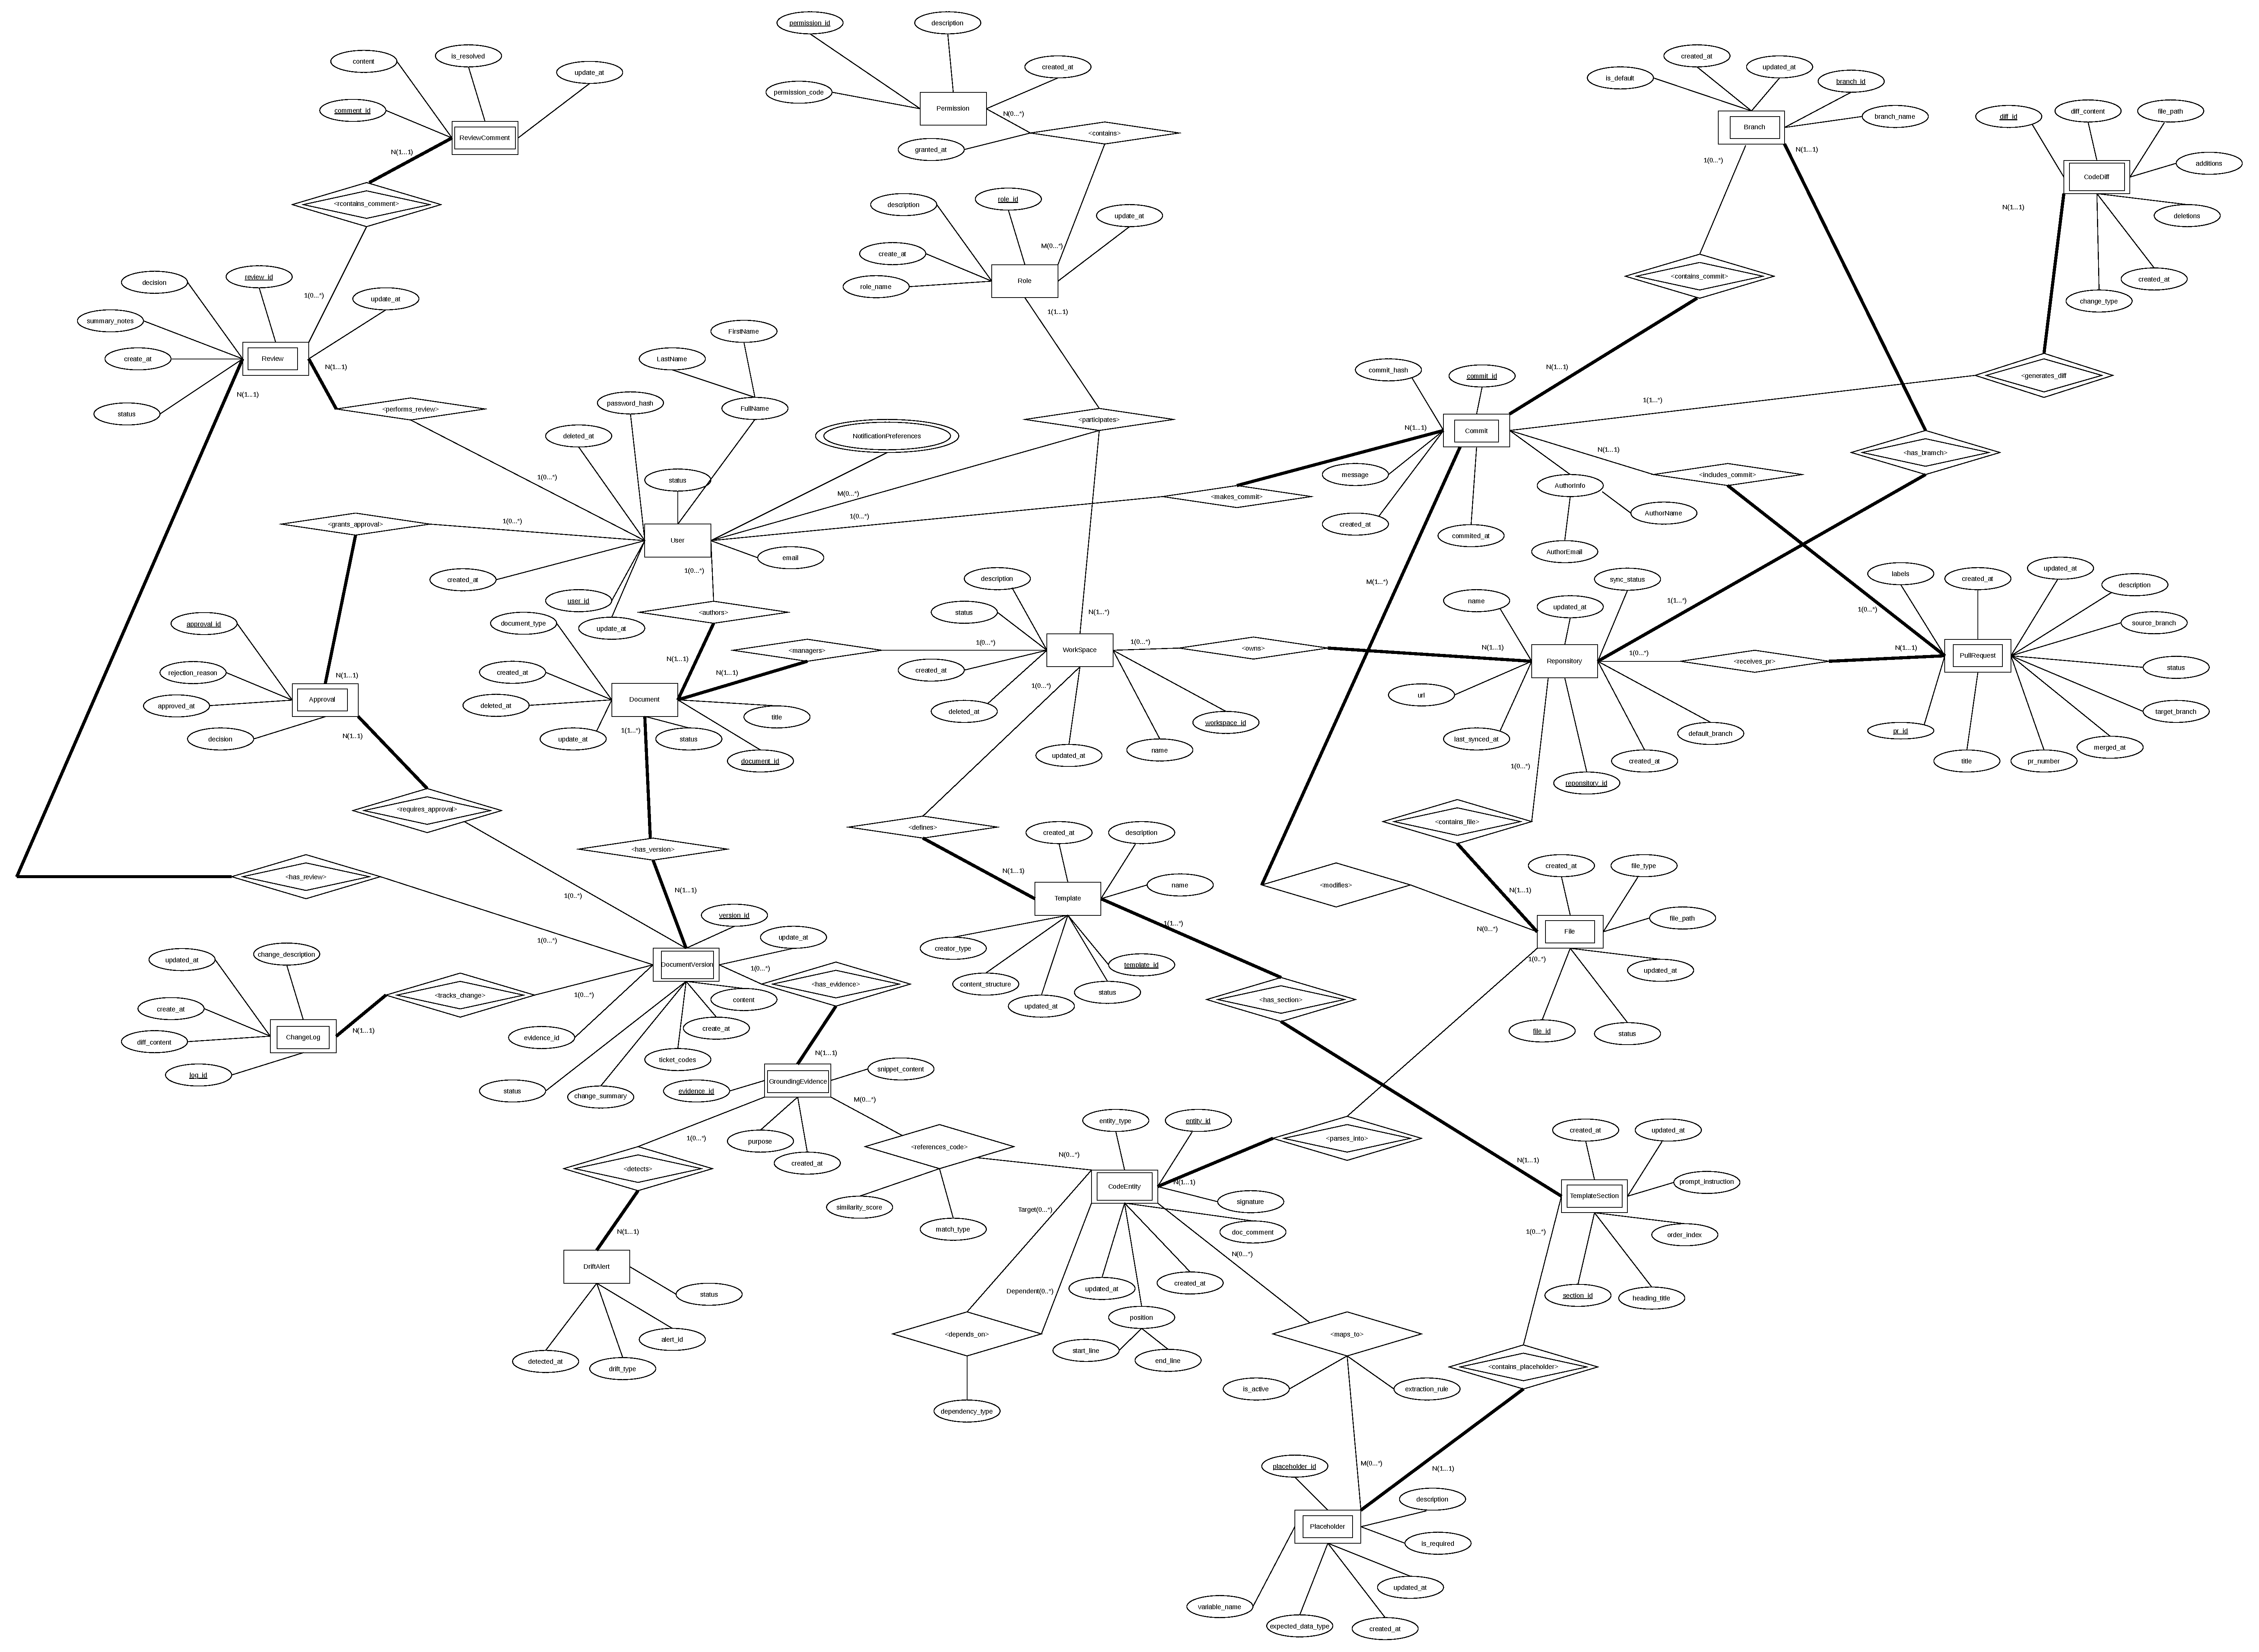
\includegraphics[
        width=\textwidth,
        height=0.75\textheight,
        keepaspectratio
    ]{./images/erd_muckhainiem.pdf}
    \caption{Sơ đồ ERD mức khái niệm}
    \label{fig:erd-conceptual}
\end{figure}
\noindent
Sơ đồ ERD mức khái niệm đã phác họa một cách toàn diện và chặt chẽ kiến trúc dữ liệu tổng quan cho Hệ thống Quản lý và Đồng bộ Tài liệu Kỹ thuật với Mã nguồn Dự án Phần mềm. Sơ đồ này không chỉ là bản thiết kế tĩnh về lưu trữ, mà còn phản ánh luồng nghiệp vụ khép kín, giải quyết bài toán cốt lõi: duy trì sự thống nhất và minh bạch giữa tài liệu kỹ thuật và mã nguồn thực tế trong suốt vòng đời phát triển phần mềm (SDLC).
Mô hình dữ liệu được phân rã một cách có hệ thống thành bốn nhóm phân hệ nghiệp vụ trọng tâm, có tính liên kết chặt chẽ với nhau:
Phân hệ Quản trị Người dùng, Định danh và Tổ chức Không gian làm việc: Hệ thống bắt đầu bằng việc thiết lập nền tảng bảo mật và tổ chức công việc đa người dùng. Cấu trúc dữ liệu cho phép xác thực người dùng chặt chẽ, gán vai trò và phân quyền truy cập chi tiết. Sau khi đăng nhập, người dùng sẽ khởi tạo và quản lý các Workspace (Không gian làm việc). Đây là các ranh giới luận lý giúp tổ chức dự án, cô lập tài nguyên và làm tiền đề cho việc tích hợp với các kho lưu trữ bên ngoài.
Phân hệ Tích hợp, Trích xuất và Quản lý Tri thức Mã nguồn: Từ không gian làm việc, các Repository (Kho chứa mã) được kết nối trực tiếp với hệ sinh thái quản lý phiên bản thông qua GitHubConnection. Luồng dữ liệu tự động đồng bộ liên tục các siêu dữ liệu quan trọng bao gồm: Branch (Nhánh phát triển), Commit (Lịch sử thay đổi), PullRequest (Yêu cầu gộp mã) và CodeDiff (Chi tiết các dòng mã thay đổi). Từ các File bị tác động, hệ thống thực hiện phân tích cú pháp để bóc tách thành các CodeEntity (Thực thể mã nguồn như hàm, lớp, biến). Các CodeEntity này đóng vai trò là lõi tri thức của hệ thống, biến mã nguồn thô thành dữ liệu có cấu trúc để sẵn sàng phục vụ cho việc sinh tài liệu.
Phân hệ Tự động Sinh tài liệu và Truy vết Bằng chứng (Traceability): Đây là trái tim của hệ thống, nơi tài liệu kỹ thuật được xây dựng không phải bằng phương pháp thủ công mà thông qua cơ chế tự động hóa dựa trên ngữ cảnh (context-aware). Hệ thống cung cấp các Template (Khuôn mẫu) được thiết kế theo các tiêu chuẩn ngành, bao gồm nhiều TemplateSection (Phân hệ nội dung) và các Placeholder (Biến định vị). Thay vì điền tay, dữ liệu từ các CodeEntity sẽ được ánh xạ động vào các Placeholder này để sinh ra các Document (Tài liệu) hoàn chỉnh. Đặc biệt, sự liên kết này được hiện thực hóa thông qua các GroundingEvidence (Bằng chứng truy vết), giúp người đọc luôn biết chính xác đoạn văn bản nào đang mô tả cho đoạn code (hoặc kiến trúc) nào, đảm bảo nội dung tài liệu luôn có cơ sở thực tế và tính chính xác tuyệt đối.
Phân hệ Kiểm soát Sai lệch (Drift Detection), Quản lý Phiên bản và Kiểm duyệt: Để giải quyết triệt để tình trạng "tài liệu bị lỗi thời", sơ đồ ERD đã định nghĩa một cơ chế giám sát vòng đời tài liệu nghiêm ngặt. Mỗi khi kho mã nguồn có biến động (commit mới), hệ thống sẽ đối chiếu và tự động phát sinh các DriftAlert (Cảnh báo sai lệch) nếu phát hiện tài liệu hiện hành không còn phản ánh đúng thực trạng mã nguồn. Mọi thay đổi trong nội dung tài liệu đều được theo dõi chặt chẽ thông qua DocumentVersion (Phiên bản tài liệu) và lưu vết tại ChangeLog (Lịch sử thay đổi). Cuối cùng, trước khi một phiên bản tài liệu được hợp thức hóa và ban hành, nó buộc phải đi qua một quy trình kiểm duyệt nhiều bước bao gồm Review (Đợt đánh giá), ReviewComment (Góp ý chi tiết) và Approval (Phê duyệt).
Nhìn một cách tổng thể, sơ đồ ERD mức khái niệm này đã tái hiện thành công một luồng dữ liệu khép kín: từ khâu tổ chức và cấp phép truy cập, đồng bộ và phân tích mã nguồn sâu, cho đến quy trình sinh tài liệu tự động hóa và giám sát vòng đời chặt chẽ. Cấu trúc dữ liệu này vượt xa yêu cầu lưu trữ thông tin đơn thuần; nó thiết lập một bộ quy tắc logic vững chắc giúp hiện thực hóa tầm nhìn của dự án là loại bỏ khoảng cách giữa code và document, đảm bảo tính đồng bộ, minh bạch và tin cậy cao nhất cho mọi dự án phần mềm.



\section{Sơ đồ Class}

\begin{figure}[H]
    \centering
    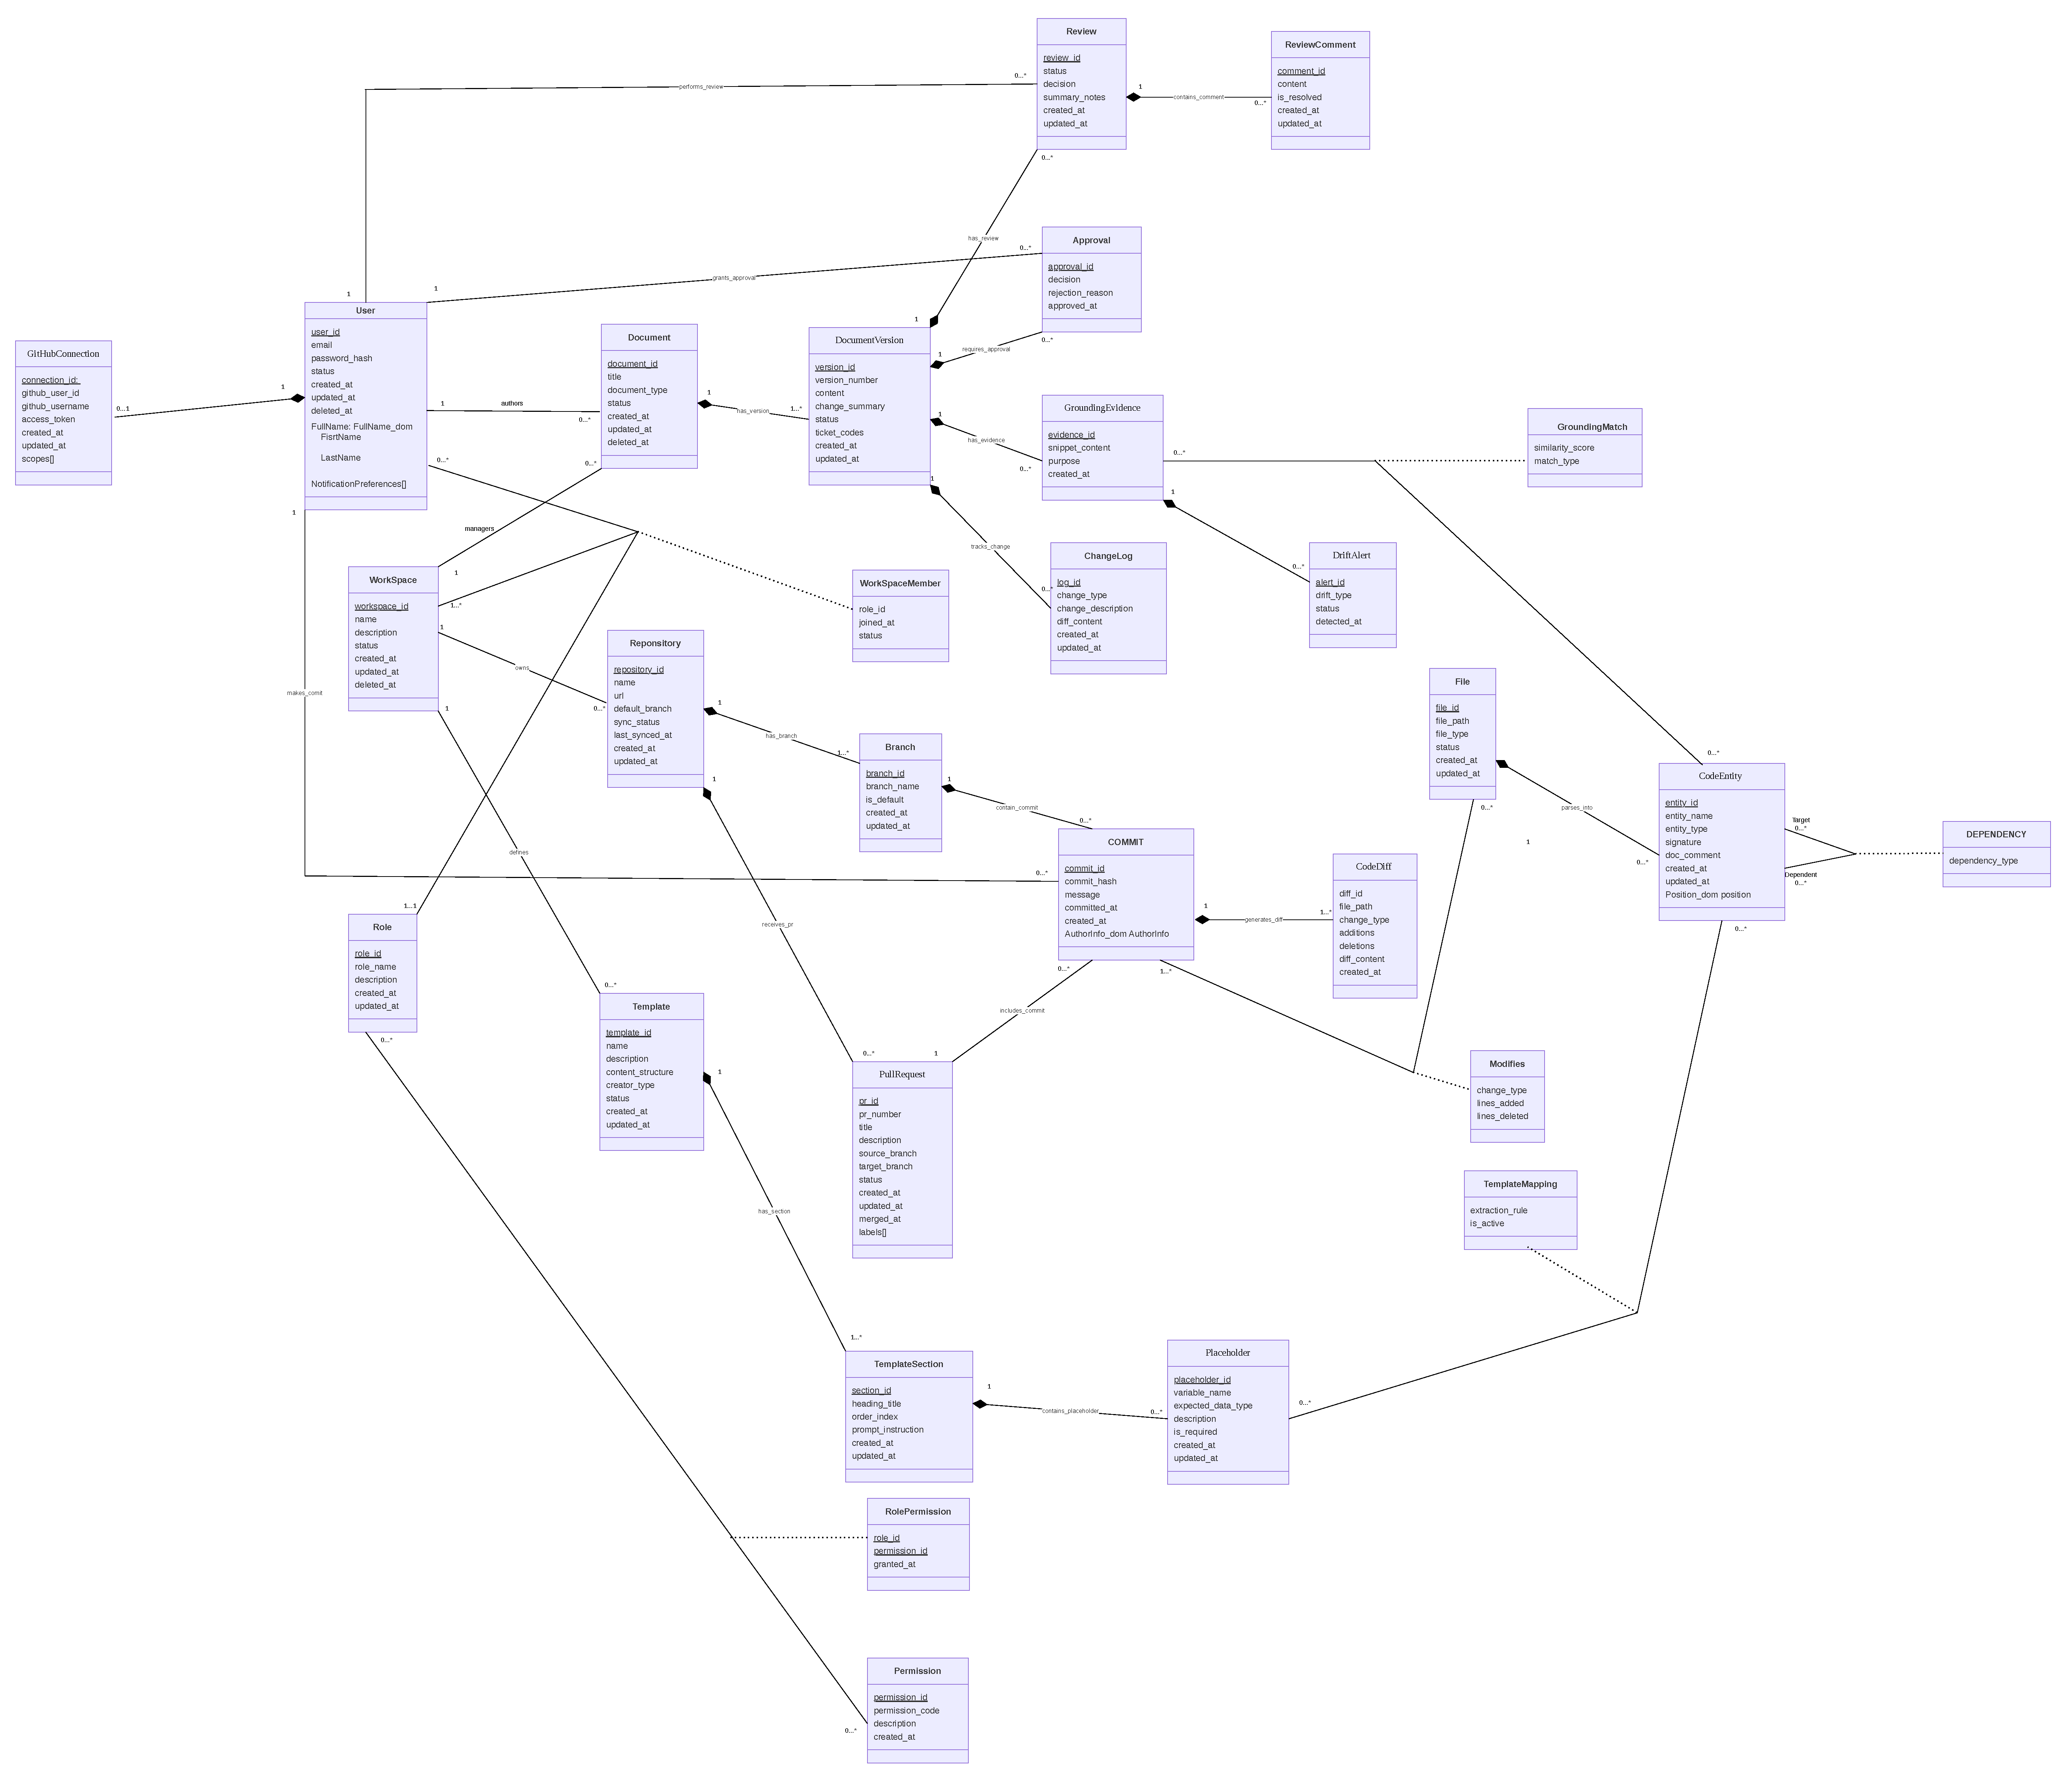
\includegraphics[
        width=\textwidth,
        height=0.75\textheight,
        keepaspectratio
    ]{./images/class.pdf}
    \caption{Sơ đồ Class}
    \label{fig:class-diagram}
\end{figure}
\noindent
Sơ đồ Lớp (Class Diagram) phác họa chi tiết cấu trúc tĩnh của tầng miền nghiệp vụ (Domain Layer) thuộc Hệ thống Quản lý và Đồng bộ Tài liệu Kỹ thuật với Mã nguồn, được phân hoạch rõ ràng thành sáu nhóm chức năng chuyên biệt. Nhóm quản trị định danh và tổ chức xoay quanh các lớp User, Role, Permission và WorkSpace, chịu trách nhiệm thiết lập bảo mật và không gian làm việc luận lý. Nhóm tích hợp mã nguồn gồm GitHubConnection, Repository, Branch, Commit, PullRequest, CodeDiff, File và CodeEntity, giúp mô hình hóa việc kết nối và đồng bộ dữ liệu từ hệ thống quản lý phiên bản. Việc định nghĩa cấu trúc tài liệu được đảm nhận bởi nhóm khuôn mẫu (Template, TemplateSection, Placeholder), trong khi nội dung thực tế và lịch sử biến động được kiểm soát chặt chẽ bởi nhóm quản lý vòng đời tài liệu (Document, DocumentVersion, ChangeLog). Quá trình kiểm soát chất lượng trước khi ban hành được chuẩn hóa qua nhóm quy trình đánh giá (Review, ReviewComment, Approval), và cuối cùng là nhóm giám sát đồng bộ (DriftAlert) giúp cảnh báo mọi sai lệch giữa tài liệu và thực trạng mã nguồn. 
Về mặt nguyên lý thiết kế hướng đối tượng, hệ thống thể hiện rõ tính đóng gói (Encapsulation) và trách nhiệm đơn lẻ (Single Responsibility), trong đó mỗi lớp chỉ nắm giữ tập thuộc tính và trạng thái thuộc phạm vi trách nhiệm của riêng mình. Thay vì để các thuộc tính rời rạc trên lớp chủ, thiết kế ưu tiên sử dụng các Đối tượng Giá trị (Value Object) như FullName\_dom, AuthorInfo\_dom hay Position\_dom để đóng gói các nhóm thuộc tính có liên quan chặt chẽ về mặt ngữ nghĩa (như họ tên, thông tin tác giả, tọa độ mã nguồn), giúp làm sạch lớp thực thể chính và tăng tính tái sử dụng. Đặc biệt, các mối quan hệ nhiều - nhiều mang thuộc tính riêng đã được mô hình hóa thành các Lớp liên kết (Association Class) độc lập như RolePermission, WorkSpaceMember, GroundingMatch, TemplateMapping, Modifies và Dependency. Kỹ thuật quan trọng này giúp tách bạch hoàn toàn bản thể dữ liệu cốt lõi khỏi siêu dữ liệu mô tả mối quan hệ, qua đó giải quyết bài toán mở rộng ngữ nghĩa (ví dụ: một biến giữ chỗ khớp với thực thể mã với độ tương đồng bao nhiêu) một cách an toàn mà không làm phình to hay rối rắm cấu trúc của các lớp gốc. 






\part{Thiết kế Logic}\label{p:second}


\chapter{Áp dụng Thuật toán 2.2 (Lược đồ Quan hệ \& Chuẩn hóa) 3NF}\label{c:figures}
Ở mức thiết kế logic (\textit{Logical Design Level}), mục tiêu cốt lõi là chuyển hóa mô hình dữ liệu quan niệm trừu tượng (ERD/UML) thành lược đồ quan hệ lô-gíc (\textit{Logical Relational Schema}) cụ thể, xác định rõ cấu trúc các bảng, cột, khóa chính (PK), khóa ngoại (FK) và các ràng buộc toàn vẹn [1, 2]. Đồ án áp dụng \textbf{Thuật toán 2.2} (\textit{Algorithm 2.2: Ánh xạ ERD sang Lược đồ Quan hệ}) để đảm bảo tính toàn vẹn tham chiếu, loại bỏ các dị thường dữ liệu và đưa toàn bộ lược đồ đạt tiêu chuẩn chuẩn hóa 3NF cho hệ thống \textbf{LivingDocs — Design and Implementation of an AI-Assisted Self-Updating Document System for Engineering Teams} [3-5].

Quá trình này tiếp nhận đầu vào (\textit{Input}) là Sơ đồ Quan niệm (\textit{Conceptual ERD/UML}) đã qua kiểm chứng ở Stage 1, và kết xuất đầu ra (\textit{Output}) là Lược đồ Quan hệ Lô-gíc (\textit{Logical Schema}) hoàn chỉnh, hồ sơ Ràng buộc Khóa ngoại/Giá trị miền (\textit{FK \& CHECK Rules}) và Báo cáo chứng minh Chuẩn hóa 3NF [3, 5-12].

\textbf{Quy trình Thuật toán 2.2 (\textit{Relational Mapping Algorithm}):}
\begin{itemize}
    \item \textbf{Đầu vào (\textit{Input}):} Sơ đồ Quan niệm ERD/UML và từ điển dữ liệu hoàn chỉnh từ Stage 1.
    \item \textbf{Bước 1 (Thực thể mạnh):} Ánh xạ các thực thể mạnh thành các bảng chính, chuyển thuộc tính đơn thành cột và thiết lập Khóa chính (PK).
    \item \textbf{Bước 2 (Thực thể yếu):} Ánh xạ các thực thể yếu thành các bảng phụ thuộc, gán Surrogate PK kiểu UUID và cài đặt FK trỏ về thực thể chủ.
    \item \textbf{Bước 3 \& 4 (Mối kết hợp $1:1$ và $1:N$):} Chèn Khóa ngoại (FK) từ bảng phía 1 sang bảng phía $N$ (hoặc phía tham gia bắt buộc) kèm các ràng buộc NOT NULL/UNIQUE phù hợp.
    \item \textbf{Bước 5 (Mối kết hợp $M:N$):} Khởi tạo các bảng trung gian (\textit{Junction Tables}) chứa cặp Khóa ngoại (FK) trỏ về hai bảng gốc và các thuộc tính riêng của mối kết hợp.
    \item \textbf{Bước 6 (Thuộc tính đặc biệt):} Phẳng hóa các thuộc tính phức hợp thành các cột đơn độc lập và tách các thuộc tính đa trị thành các bảng phụ riêng.
    \item \textbf{Bước 7 (Ràng buộc \& Chuẩn hóa):} Khai báo tập Phụ thuộc hàm (FDs), chứng minh lược đồ đạt chuẩn 3NF và thiết lập các ràng buộc toàn vẹn (\textit{FK Constraints}).
    \item \textbf{Đầu ra (\textit{Output}):} Lược đồ Quan hệ Lô-gíc (\textit{Logical Schema}) hoàn chỉnh đạt chuẩn 3NF và hồ sơ ràng buộc toàn vẹn.
\end{itemize}

\section{ Ánh xạ Thực thể, Mối kết hợp \& Phẳng hóa Thuộc tính (Thuật toán 2.2) }



\subsubsection*{Bước 1: Thực thể mạnh $\rightarrow$ Bảng chính}
Chuyển 7 thực thể mạnh thành 7 bảng chính, đặt tên theo chuẩn \texttt{snake\_case} số nhiều:
\begin{itemize}
    \item \texttt{users}, \texttt{workspaces}, \texttt{roles}, \texttt{permissions}, \texttt{repositories}, \texttt{templates}, \texttt{documents}.
\end{itemize}

\subsubsection*{Bước 2: Thực thể yếu $\rightarrow$ Bảng phụ \& Mối kết hợp $M:N \rightarrow$ Bảng trung gian (Surrogate PK UUID)}
Chuyển 16 thực thể yếu thành 16 bảng phụ, mỗi bảng được gán khóa chính nhân tạo (Surrogate PK) kiểu \texttt{UUID} độc lập với bảng cha, mang FK định danh (identifying FK) trỏ về đúng 1 bảng cha:
\begin{itemize}
    \item \texttt{github\_connections} (phụ thuộc \texttt{users})
    \item \texttt{branches} (phụ thuộc \texttt{repositories})
    \item \texttt{commits} (phụ thuộc \texttt{branches}; FK phụ \texttt{author\_user\_id} $\rightarrow$ \texttt{users}, \texttt{pr\_id} $\rightarrow$ \texttt{pull\_requests})
    \item \texttt{pull\_requests} (phụ thuộc \texttt{repositories})
    \item \texttt{code\_diffs} (phụ thuộc \texttt{commits})
    \item \texttt{files} (phụ thuộc \texttt{repositories})
    \item \texttt{code\_entities} (phụ thuộc \texttt{files})
    \item \texttt{template\_sections} (phụ thuộc \texttt{templates})
    \item \texttt{placeholders} (phụ thuộc \texttt{template\_sections})
    \item \texttt{document\_versions} (phụ thuộc \texttt{documents})
    \item \texttt{change\_logs} (phụ thuộc \texttt{document\_versions})
    \item \texttt{reviews} (phụ thuộc \texttt{document\_versions}; FK phụ \texttt{reviewer\_user\_id} $\rightarrow$ \texttt{users})
    \item \texttt{review\_comments} (phụ thuộc \texttt{reviews})
    \item \texttt{approvals} (phụ thuộc \texttt{document\_versions}; FK phụ \texttt{approver\_user\_id} $\rightarrow$ \texttt{users})
    \item \texttt{grounding\_evidences} (phụ thuộc \texttt{document\_versions})
    \item \texttt{drift\_alerts} (phụ thuộc \texttt{grounding\_evidences})
\end{itemize}

Song song đó, chuyển các mối kết hợp $M:N$ (bao gồm 1 mối kết hợp 3 ngôi và 1 mối kết hợp đệ quy) thành 6 bảng trung gian, mỗi bảng được gán Surrogate PK riêng kiểu \texttt{UUID}, chứa tối thiểu 2 FK cùng vai trò định danh trỏ về các bảng gốc:
\begin{itemize}
    \item \texttt{workspace\_members} (mối kết hợp 3 ngôi \textit{participates}: \texttt{user\_id}, \texttt{workspace\_id}, \texttt{role\_id})
    \item \texttt{role\_permissions} (mối kết hợp \textit{contains}: \texttt{role\_id}, \texttt{permission\_id})
    \item \texttt{commit\_file} (mối kết hợp \textit{modifies}: \texttt{commit\_id}, \texttt{file\_id})
    \item \texttt{dependencies} (mối kết hợp đệ quy \textit{depends\_on}: \texttt{dependent\_entity\_id}, \texttt{target\_entity\_id} --- cả hai cùng trỏ về \texttt{code\_entities})
    \item \texttt{template\_mappings} (mối kết hợp \textit{maps\_to}: \texttt{placeholder\_id}, \texttt{code\_entity\_id})
    \item \texttt{grounding\_evidence\_code\_entities} (mối kết hợp \textit{references\_code}: \texttt{evidence\_id}, \texttt{code\_entity\_id})
\end{itemize}

\subsubsection*{Bước 3 \& 4: Quan hệ 1:1, 1:N $\rightarrow$ Chèn FK}
\textbf{Nguyên tắc:} Chuyển khóa chính (PK) của bảng phía 1 sang làm khóa ngoại (FK) ở bảng phía N. Với quan hệ 1:1, đặt khóa ngoại ở phía tham gia tùy chọn và gán ràng buộc \texttt{UNIQUE} để đảm bảo tính một-một.
\begin{itemize}
    \item \texttt{users.user\_id} (PK) $\rightarrow$ \texttt{github\_connections.user\_id} (FK) (1:1 nghiệp vụ, ràng buộc \texttt{UNIQUE})
    \item \texttt{workspaces.workspace\_id} (PK) $\rightarrow$ \texttt{repositories.workspace\_id} (FK) (1:N)
    \item \texttt{repositories.repository\_id} (PK) $\rightarrow$ \texttt{branches.repository\_id} (FK) (1:N)
    \item \texttt{branches.branch\_id} (PK) $\rightarrow$ \texttt{commits.branch\_id} (FK) (1:N)
    \item \texttt{commits.author\_user\_id} (FK) $\rightarrow$ \texttt{users.user\_id} (PK) (1:N)
    \item \texttt{commits.pr\_id} (FK) $\rightarrow$ \texttt{pull\_requests.pr\_id} (PK) (1:N, cho phép NULL)
    \item \texttt{pull\_requests.repository\_id} (FK) $\rightarrow$ \texttt{repositories.repository\_id} (PK) (1:N)
    \item \texttt{code\_diffs.commit\_id} (FK) $\rightarrow$ \texttt{commits.commit\_id} (PK) (1:N)
    \item \texttt{files.repository\_id} (FK) $\rightarrow$ \texttt{repositories.repository\_id} (PK) (1:N)
    \item \texttt{code\_entities.file\_id} (FK) $\rightarrow$ \texttt{files.file\_id} (PK) (1:N)
    \item \texttt{templates.workspace\_id} (FK) $\rightarrow$ \texttt{workspaces.workspace\_id} (PK) (1:N)
    \item \texttt{template\_sections.template\_id} (FK) $\rightarrow$ \texttt{templates.template\_id} (PK) (1:N)
    \item \texttt{placeholders.section\_id} (FK) $\rightarrow$ \texttt{template\_sections.section\_id} (PK) (1:N)
    \item \texttt{documents.workspace\_id} (FK) $\rightarrow$ \texttt{workspaces.workspace\_id} (PK) (1:N)
    \item \texttt{documents.author\_user\_id} (FK) $\rightarrow$ \texttt{users.user\_id} (PK) (1:N)
    \item \texttt{document\_versions.document\_id} (FK) $\rightarrow$ \texttt{documents.document\_id} (PK) (1:N)
    \item \texttt{change\_logs.version\_id} (FK) $\rightarrow$ \texttt{document\_versions.version\_id} (PK) (1:N)
    \item \texttt{reviews.version\_id} (FK) $\rightarrow$ \texttt{document\_versions.version\_id} (PK) (1:N)
    \item \texttt{reviews.reviewer\_user\_id} (FK) $\rightarrow$ \texttt{users.user\_id} (PK) (1:N)
    \item \texttt{review\_comments.review\_id} (FK) $\rightarrow$ \texttt{reviews.review\_id} (PK) (1:N)
    \item \texttt{approvals.version\_id} (FK) $\rightarrow$ \texttt{document\_versions.version\_id} (PK) (1:N)
    \item \texttt{approvals.approver\_user\_id} (FK) $\rightarrow$ \texttt{users.user\_id} (PK) (1:N)
    \item \texttt{grounding\_evidences.version\_id} (FK) $\rightarrow$ \texttt{document\_versions.version\_id} (PK) (1:N)
    \item \texttt{drift\_alerts.evidence\_id} (FK) $\rightarrow$ \texttt{grounding\_evidences.evidence\_id} (PK) (1:N)
\end{itemize}

\subsubsection*{Bước 5: Quan hệ M:N $\rightarrow$ Bảng trung gian}
Tạo 6 bảng trung gian, mỗi bảng có Surrogate PK riêng kiểu \texttt{UUID} và tối thiểu 2 FK trỏ về các bảng gốc:
\begin{itemize}
    \item \texttt{workspace\_members}: chứa FK \texttt{user\_id}, \texttt{workspace\_id}, \texttt{role\_id} (mối kết hợp 3 ngôi \textit{participates}, tỷ lệ M:N:1)
    \item \texttt{role\_permissions}: chứa FK \texttt{role\_id}, \texttt{permission\_id} (mối kết hợp \textit{contains}, M:N)
    \item \texttt{commit\_file}: chứa FK \texttt{commit\_id}, \texttt{file\_id} (mối kết hợp \textit{modifies}, M:N)
    \item \texttt{dependencies}: chứa FK \texttt{dependent\_entity\_id}, \texttt{target\_entity\_id} (mối kết hợp đệ quy \textit{depends\_on}, M:N)
    \item \texttt{template\_mappings}: chứa FK \texttt{placeholder\_id}, \texttt{code\_entity\_id} (mối kết hợp \textit{maps\_to}, M:N)
    \item \texttt{grounding\_evidence\_code\_entities}: chứa FK \texttt{evidence\_id}, \texttt{code\_entity\_id} (mối kết hợp \textit{references\_code}, M:N)
\end{itemize}

\subsubsection*{Bước 6: Thuộc tính đặc biệt}
\begin{itemize}
    \item \textbf{Phẳng hóa thuộc tính phức hợp:}
    \begin{itemize}
        \item \texttt{User.FullName} $\rightarrow$ \texttt{users.first\_name}, \texttt{users.last\_name}
        \item \texttt{Commit.AuthorInfo} $\rightarrow$ \texttt{commits.author\_name}, \texttt{commits.author\_email}
        \item \texttt{CodeEntity.position} $\rightarrow$ \texttt{code\_entities.start\_line}, \texttt{code\_entities.end\_line}
    \end{itemize}
    \item \textbf{Tách thuộc tính đa trị thành bảng phụ chứa FK trỏ về bảng chính:}
    \begin{itemize}
        \item \texttt{User.NotificationPreferences} $\rightarrow$ \texttt{user\_notification\_preferences}
        \item \texttt{GitHubConnection.scopes} $\rightarrow$ \texttt{github\_connection\_scopes}
        \item \texttt{PullRequest.labels} $\rightarrow$ \texttt{pull\_request\_labels}
    \end{itemize}
\end{itemize};

% ==========================================
\section{ Lược đồ Quan hệ Lô-gíc (Logical Schema) \& 3NF-Phân hệ Quản trị \& Xác thực}


\paragraph{1. Bảng \texttt{users}} (Bảng chính - Thực thể mạnh: User)
\begin{table}[H]
\centering
\begin{tabular}{|l|l|c|l|}
\hline
\textbf{Tên Cột} & \textbf{Kiểu Dữ Liệu} & \textbf{Khóa} & \textbf{Ràng Buộc} \\ \hline
\texttt{user\_id} & UUID & PK & NOT NULL \\ \hline
\texttt{email} & - & Unique & NOT NULL \\ \hline
\texttt{password\_hash} & - & - & NULL \\ \hline
\texttt{first\_name} & - & - & NULL \\ \hline
\texttt{last\_name} & - & - & NULL \\ \hline
\texttt{status} & - & - & NOT NULL \\ \hline
\texttt{created\_at} & - & - & NOT NULL \\ \hline
\texttt{updated\_at} & - & - & NOT NULL \\ \hline
\texttt{deleted\_at} & - & - & NULL \\ \hline
\end{tabular}
\end{table}

\paragraph{2. Bảng \texttt{workspaces}} (Bảng chính - Thực thể mạnh: Workspace)
\begin{table}[H]
\centering
\begin{tabular}{|l|l|c|l|}
\hline
\textbf{Tên Cột} & \textbf{Kiểu Dữ Liệu} & \textbf{Khóa} & \textbf{Ràng Buộc} \\ \hline
\texttt{workspace\_id} & UUID & PK & NOT NULL \\ \hline
\texttt{name} & - & - & NOT NULL \\ \hline
\texttt{description} & - & - & NULL \\ \hline
\texttt{status} & - & - & NOT NULL \\ \hline
\texttt{created\_at} & - & - & NOT NULL \\ \hline
\texttt{updated\_at} & - & - & NOT NULL \\ \hline
\texttt{deleted\_at} & - & - & NULL \\ \hline
\end{tabular}
\end{table}

\paragraph{3. Bảng \texttt{roles}} (Bảng chính - Thực thể mạnh: Role)
\begin{table}[H]
\centering
\begin{tabular}{|l|l|c|l|}
\hline
\textbf{Tên Cột} & \textbf{Kiểu Dữ Liệu} & \textbf{Khóa} & \textbf{Ràng Buộc} \\ \hline
\texttt{role\_id} & UUID & PK & NOT NULL \\ \hline
\texttt{role\_name} & - & - & NOT NULL \\ \hline
\texttt{description} & - & - & NULL \\ \hline
\texttt{created\_at} & - & - & NOT NULL \\ \hline
\texttt{updated\_at} & - & - & NOT NULL \\ \hline
\end{tabular}
\end{table}

\paragraph{4. Bảng \texttt{permissions}} (Bảng chính - Thực thể mạnh: Permission)
\begin{table}[H]
\centering
\begin{tabular}{|l|l|c|l|}
\hline
\textbf{Tên Cột} & \textbf{Kiểu Dữ Liệu} & \textbf{Khóa} & \textbf{Ràng Buộc} \\ \hline
\texttt{permission\_id} & UUID & PK & NOT NULL \\ \hline
\texttt{permission\_code} & - & Unique & NOT NULL \\ \hline
\texttt{description} & - & - & NULL \\ \hline
\texttt{created\_at} & - & - & NOT NULL \\ \hline
\end{tabular}
\end{table}

\paragraph{5. Bảng \texttt{github\_connections}} (Bảng phụ - Thực thể yếu phụ thuộc User, Surrogate PK UUID)
\begin{table}[H]
\centering
\begin{tabular}{|l|l|c|l|}
\hline
\textbf{Tên Cột} & \textbf{Kiểu Dữ Liệu} & \textbf{Khóa} & \textbf{Ràng Buộc} \\ \hline
\texttt{connection\_id} & UUID & PK & NOT NULL \\ \hline
\texttt{user\_id} & - & FK, Unique & NOT NULL \\ \hline
\texttt{github\_user\_id} & - & - & NOT NULL \\ \hline
\texttt{github\_username} & - & - & NOT NULL \\ \hline
\texttt{access\_token} & - & - & NOT NULL \\ \hline
\texttt{created\_at} & - & - & NOT NULL \\ \hline
\texttt{updated\_at} & - & - & NOT NULL \\ \hline
\multicolumn{4}{|l|}{\textbf{Ràng buộc bổ sung:} \texttt{UNIQUE (user\_id)}} \\ \hline
\end{tabular}
\end{table}

\paragraph{6. Bảng \texttt{user\_notification\_preferences}} (Bảng phụ đa trị từ \texttt{NotificationPreferences} của User)
\begin{table}[H]
\centering
\begin{tabular}{|l|l|c|l|}
\hline
\textbf{Tên Cột} & \textbf{Kiểu Dữ Liệu} & \textbf{Khóa} & \textbf{Ràng Buộc} \\ \hline
\texttt{preference\_id} & UUID & PK & NOT NULL \\ \hline
\texttt{user\_id} & - & FK & NOT NULL \\ \hline
\texttt{channel} & - & - & NOT NULL \\ \hline
\multicolumn{4}{|l|}{\textbf{Ràng buộc bổ sung:} \texttt{UNIQUE (user\_id, channel)}} \\
\multicolumn{4}{|l|}{\textit{Một người dùng chỉ có tối đa 1 bản ghi cho mỗi kênh.}} \\ \hline
\end{tabular}
\end{table}

\paragraph{7. Bảng \texttt{github\_connection\_scopes}} (Bảng phụ đa trị từ \texttt{scopes} của GitHubConnection)
\begin{table}[H]
\centering
\begin{tabular}{|l|l|c|l|}
\hline
\textbf{Tên Cột} & \textbf{Kiểu Dữ Liệu} & \textbf{Khóa} & \textbf{Ràng Buộc} \\ \hline
\texttt{scope\_id} & UUID & PK & NOT NULL \\ \hline
\texttt{connection\_id} & - & FK & NOT NULL \\ \hline
\texttt{scope\_value} & - & - & NOT NULL \\ \hline
\multicolumn{4}{|l|}{\textbf{Ràng buộc bổ sung:} \texttt{UNIQUE (connection\_id, scope\_value)}} \\
\multicolumn{4}{|l|}{\textit{Đảm bảo tài khoản OAuth không lưu lặp lại cùng một quyền scope.}} \\ \hline
\end{tabular}
\end{table}

\paragraph{8. Bảng \texttt{workspace\_members}} (Bảng trung gian mối kết hợp 3 ngôi User–Workspace–Role, tỷ lệ M:N:1)
\begin{table}[H]
\centering
\begin{tabular}{|l|l|c|l|}
\hline
\textbf{Tên Cột} & \textbf{Kiểu Dữ Liệu} & \textbf{Khóa} & \textbf{Ràng Buộc} \\ \hline
\texttt{membership\_id} & UUID & PK & NOT NULL \\ \hline
\texttt{user\_id} & - & FK & NOT NULL \\ \hline
\texttt{workspace\_id} & - & FK & NOT NULL \\ \hline
\texttt{role\_id} & - & FK & NOT NULL \\ \hline
\texttt{joined\_at} & - & - & NOT NULL \\ \hline
\texttt{status} & - & - & NOT NULL \\ \hline
\multicolumn{4}{|l|}{\textbf{Ràng buộc bổ sung:} \texttt{UNIQUE (user\_id, workspace\_id)}} \\
\multicolumn{4}{|l|}{\textit{Đảm bảo mỗi User chỉ giữ đúng 1 Role trong 1 Workspace (Scoped RBAC).}} \\ \hline
\end{tabular}
\end{table}

\paragraph{9. Bảng \texttt{role\_permissions}} (Bảng trung gian mối kết hợp Role–Permission, tỷ lệ M:N)
\begin{table}[H]
\centering
\begin{tabular}{|l|l|c|l|}
\hline
\textbf{Tên Cột} & \textbf{Kiểu Dữ Liệu} & \textbf{Khóa} & \textbf{Ràng Buộc} \\ \hline
\texttt{role\_permission\_id} & UUID & PK & NOT NULL \\ \hline
\texttt{role\_id} & - & FK & NOT NULL \\ \hline
\texttt{permission\_id} & - & FK & NOT NULL \\ \hline
\texttt{granted\_at} & - & - & NOT NULL \\ \hline
\multicolumn{4}{|l|}{\textbf{Ràng buộc bổ sung:} \texttt{UNIQUE (role\_id, permission\_id)}} \\
\multicolumn{4}{|l|}{\textit{Ngăn chặn gán trùng lặp quyền cho một vai trò (RBAC).}} \\ \hline
\end{tabular}
\end{table}
\subsection{Lược đồ Cú pháp Rút gọn \& Chứng minh Chuẩn hóa 3NF}

\subsubsection{Lược đồ Dạng Cú pháp Rút gọn}

\begin{itemize}
    \item \texttt{users} (\underline{\texttt{user\_id}} [UUID, PK], \texttt{email} [Unique], \texttt{password\_hash}, \texttt{first\_name}, \texttt{last\_name}, \texttt{status}, \texttt{created\_at}, \texttt{updated\_at}, \texttt{deleted\_at})
    \item \texttt{workspaces} (\underline{\texttt{workspace\_id}} [UUID, PK], \texttt{name}, \texttt{description}, \texttt{status}, \texttt{created\_at}, \texttt{updated\_at}, \texttt{deleted\_at})
    \item \texttt{roles} (\underline{\texttt{role\_id}} [UUID, PK], \texttt{role\_name}, \texttt{description}, \texttt{created\_at}, \texttt{updated\_at})
    \item \texttt{permissions} (\underline{\texttt{permission\_id}} [UUID, PK], \texttt{permission\_code} [Unique], \texttt{description}, \texttt{created\_at})
    \item \texttt{github\_connections} (\underline{\texttt{connection\_id}} [UUID, PK], \texttt{user\_id} [FK, Unique], \texttt{github\_user\_id}, \texttt{github\_username}, \texttt{access\_token}, \texttt{created\_at}, \texttt{updated\_at})
    \item \texttt{user\_notification\_preferences} (\underline{\texttt{preference\_id}} [UUID, PK], \texttt{user\_id} [FK], \texttt{channel}, \texttt{UNIQUE(user\_id, channel)})
    \item \texttt{github\_connection\_scopes} (\underline{\texttt{scope\_id}} [UUID, PK], \texttt{connection\_id} [FK], \texttt{scope\_value}, \texttt{UNIQUE(connection\_id, scope\_value)})
    \item \texttt{workspace\_members} (\underline{\texttt{membership\_id}} [UUID, PK], \texttt{user\_id} [FK], \texttt{workspace\_id} [FK], \texttt{role\_id} [FK], \texttt{joined\_at}, \texttt{status}, \texttt{UNIQUE(user\_id, workspace\_id)})
    \item \texttt{role\_permissions} (\underline{\texttt{role\_permission\_id}} [UUID, PK], \texttt{role\_id} [FK], \texttt{permission\_id} [FK], \texttt{granted\_at}, \texttt{UNIQUE(role\_id, permission\_id)})
\end{itemize}

% ==========================================
\subsection{Báo cáo Chứng minh Chuẩn hóa 3NF}

\subsubsection{Khai báo Tập Phụ thuộc Hàm (Functional Dependencies - FDs)}
Xét các bảng trong phân hệ Quản trị, Người dùng \& Phân quyền có tập phụ thuộc hàm được xác định chi tiết như sau:

\paragraph{1. Bảng \texttt{users}}
\begin{itemize}
    \item $f_1: \text{user\_id} \rightarrow \text{email, password\_hash, first\_name, last\_name, status, created\_at, updated\_at, deleted\_at}$
    \item $f_2: \text{email} \rightarrow \text{user\_id, password\_hash, first\_name, last\_name, status, created\_at, updated\_at, deleted\_at}$ \textit{(Khóa ứng viên)}
\end{itemize}

\paragraph{2. Bảng \texttt{user\_notification\_preferences}}
\begin{itemize}
    \item $f_1: \text{preference\_id} \rightarrow \text{user\_id, channel}$
    \item $f_2: (\text{user\_id, channel}) \rightarrow \text{preference\_id}$
\end{itemize}

\paragraph{3. Bảng \texttt{workspaces}}
\begin{itemize}
    \item $f_1: \text{workspace\_id} \rightarrow \text{name, description, status, created\_at, updated\_at, deleted\_at}$
\end{itemize}

\paragraph{4. Bảng \texttt{roles}}
\begin{itemize}
    \item $f_1: \text{role\_id} \rightarrow \text{role\_name, description, created\_at, updated\_at}$
\end{itemize}

\paragraph{5. Bảng \texttt{permissions}}
\begin{itemize}
    \item $f_1: \text{permission\_id} \rightarrow \text{permission\_code, description, created\_at}$
    \item $f_2: \text{permission\_code} \rightarrow \text{permission\_id, description, created\_at}$ \textit{(Khóa ứng viên)}
\end{itemize}

\paragraph{6. Bảng \texttt{role\_permissions}}
\begin{itemize}
    \item $f_1: \text{role\_permission\_id} \rightarrow \text{role\_id, permission\_id, granted\_at}$
    \item $f_2: (\text{role\_id, permission\_id}) \rightarrow \text{role\_permission\_id, granted\_at}$
\end{itemize}

\paragraph{7. Bảng \texttt{workspace\_members}}
\begin{itemize}
    \item $f_1: \text{membership\_id} \rightarrow \text{user\_id, workspace\_id, role\_id, joined\_at, status}$
    \item $f_2: (\text{user\_id, workspace\_id}) \rightarrow \text{membership\_id, role\_id, joined\_at, status}$
\end{itemize}

\paragraph{8. Bảng \texttt{github\_connections}}
\begin{itemize}
    \item $f_1: \text{connection\_id} \rightarrow \text{user\_id, github\_user\_id, github\_username, access\_token, created\_at, updated\_at}$
    \item $f_2: \text{user\_id} \rightarrow \text{connection\_id, github\_user\_id, github\_username, access\_token, created\_at, updated\_at}$ \textit{(Khóa ứng viên)}
\end{itemize}

\paragraph{9. Bảng \texttt{github\_connection\_scopes}}
\begin{itemize}
    \item $f_1: \text{scope\_id} \rightarrow \text{connection\_id, scope\_value}$
    \item $f_2: (\text{connection\_id, scope\_value}) \rightarrow \text{scope\_id}$
\end{itemize}

\subsubsection{Đánh giá Cấp Chuẩn (Normal Forms Assessment)}

\begin{itemize}
    \item \textbf{Đạt Chuẩn 1NF (First Normal Form):}
    \begin{itemize}
        \item \textit{Giá trị nguyên tố (Atomic Values):} Toàn bộ các cột trong tất cả các bảng đều lưu giữ giá trị đơn, không thể phân chia nhỏ hơn.
        \item \textit{Phẳng hóa thuộc tính phức hợp:} Thuộc tính phức hợp \texttt{FullName} đã được tách thành hai thuộc tính nguyên tố là \texttt{first\_name} và \texttt{last\_name}.
        \item \textit{Tách thuộc tính đa trị:} Các thuộc tính đa trị như danh sách cài đặt thông báo (\texttt{NotificationPreferences}) và danh sách quyền truy cập (\texttt{scopes}) đã được tách thành các bảng phụ tương ứng là \texttt{user\_notification\_preferences} và \texttt{github\_connection\_scopes}.
    \end{itemize}

    \item \textbf{Đạt Chuẩn 2NF (Second Normal Form):}
    \begin{itemize}
        \item \textit{Sử dụng Khóa chính đơn (Surrogate PK):} Mọi bảng trong phân hệ đều thiết lập Khóa chính đơn định danh bằng chuỗi UUID (\texttt{user\_id}, \texttt{workspace\_id}, \texttt{role\_id}, \texttt{membership\_id},...).
        \item \textit{Loại bỏ phụ thuộc một phần:} Do không dùng Khóa chính phức hợp làm khóa chính duy nhất, mọi thuộc tính không khóa đều phụ thuộc đầy đủ vào toàn bộ Khóa chính, loại bỏ hoàn toàn hiện tượng phụ thuộc một phần (Partial Dependency).
    \end{itemize}

    \item \textbf{Đạt Chuẩn 3NF (Third Normal Form):}
    \begin{itemize}
        \item \textit{Phụ thuộc trực tiếp:} Tất cả thuộc tính không khóa đều phụ thuộc trực tiếp vào Khóa chính của bảng chứa nó.
        \item \textit{Loại bỏ phụ thuộc bắc cầu:} Không tồn tại phụ thuộc bắc cầu dạng $X \rightarrow Y \rightarrow Z$ giữa các thuộc tính không khóa. Ví dụ: Thông tin phân quyền giữa nhóm quyền và người dùng không lưu trực tiếp trong \texttt{users} hay \texttt{roles} mà được tách riêng thành các bảng trung gian \texttt{role\_permissions} và \texttt{workspace\_members}.
    \end{itemize}
\end{itemize}
\setcounter{subsection}{1} % Ép subsection tiếp theo thành số 2 (tức là 3.2)
\section{Lược đồ Quan hệ Lô-gíc (Logical Schema) \& 3NF-Phân hệ Mã nguồn \& Cấu trúc Code}

\subsection*{Khai báo Chi tiết Bảng }

% Bảng repositories
\noindent\textbf{Tên Bảng: repositories} \par\vspace{0.1cm}
\begin{tabular}{|l|l|c|c|}
\hline
\textbf{Tên Cột} & \textbf{Kiểu Dữ liệu} & \textbf{Khóa} & \textbf{Ràng Buộc} \\
\hline
repository\_id & UUID & PK & NOT NULL \\
\hline
workspace\_id &  & FK & NOT NULL \\
\hline
name & & & NOT NULL \\
\hline
url & & Unique & NOT NULL \\
\hline
default\_branch & & & NOT NULL \\
\hline
sync\_status & & & NOT NULL \\
\hline
last\_synced\_at & & & NULL \\
\hline
created\_at & & & NOT NULL \\
\hline
updated\_at & & & NOT NULL \\
\hline
\end{tabular}
\vspace{0.4cm}

% Bảng branches
\noindent\textbf{Tên Bảng: branches} \par\vspace{0.1cm}
\begin{tabular}{|l|l|c|c|}
\hline
\textbf{Tên Cột} & \textbf{Kiểu Dữ liệu} & \textbf{Khóa} & \textbf{Ràng Buộc} \\
\hline
branch\_id & UUID & PK & NOT NULL \\
\hline
repository\_id &  & FK & NOT NULL \\
\hline
branch\_name & & & NOT NULL \\
\hline
is\_default & & & NOT NULL \\
\hline
created\_at & & & NOT NULL \\
\hline
updated\_at & & & NOT NULL \\
\hline
\end{tabular}
\vspace{0.4cm}

% Bảng commits
\noindent\textbf{Tên Bảng: commits} \par\vspace{0.1cm}
\begin{tabular}{|l|l|c|c|}
\hline
\textbf{Tên Cột} & \textbf{Kiểu Dữ liệu} & \textbf{Khóa} & \textbf{Ràng Buộc} \\
\hline
commit\_id & UUID & PK & NOT NULL \\
\hline
branch\_id &  & FK & NOT NULL \\
\hline
user\_id &  & FK & NULL \\
\hline
commit\_hash & & Unique & NOT NULL \\
\hline
message & & & NOT NULL \\
\hline
author\_name & & & NOT NULL \\
\hline
author\_email & & & NOT NULL \\
\hline
committed\_at & & & NOT NULL \\
\hline
created\_at & & & NOT NULL \\
\hline
\end{tabular}
\vspace{0.4cm}

% Bảng pull_requests
\noindent\textbf{Tên Bảng: pull\_requests} \par\vspace{0.1cm}
\begin{tabular}{|l|l|c|c|}
\hline
\textbf{Tên Cột} & \textbf{Kiểu Dữ liệu} & \textbf{Khóa} & \textbf{Ràng Buộc} \\
\hline
pr\_id & UUID & PK & NOT NULL \\
\hline
repository\_id &  & FK & NOT NULL \\
\hline
pr\_number & & & NOT NULL \\
\hline
title & & & NOT NULL \\
\hline
description & & & NOT NULL \\
\hline
source\_branch & & & NOT NULL \\
\hline
target\_branch & & & NOT NULL \\
\hline
status & & & NOT NULL \\
\hline
created\_at & & & NOT NULL \\
\hline
updated\_at & & & NOT NULL \\
\hline
merged\_at & & & NULL \\
\hline
\end{tabular}
\vspace{0.4cm}

% Bảng pull_request_labels
\noindent\textbf{Tên Bảng: pull\_request\_labels} \par\vspace{0.1cm}
\begin{tabular}{|l|l|c|c|}
\hline
\textbf{Tên Cột} & \textbf{Kiểu Dữ liệu} & \textbf{Khóa} & \textbf{Ràng Buộc} \\
\hline
label\_id & UUID & PK & NOT NULL \\
\hline
pr\_id & & FK & NOT NULL \\
\hline
label\_name & & & NOT NULL \\
\hline
\end{tabular}
\vspace{0.4cm}

% Bảng code_diffs
\noindent\textbf{Tên Bảng: code\_diffs} \par\vspace{0.1cm}
\begin{tabular}{|l|l|c|c|}
\hline
\textbf{Tên Cột} & \textbf{Kiểu Dữ liệu} & \textbf{Khóa} & \textbf{Ràng Buộc} \\
\hline
diff\_id & UUID & PK & NOT NULL \\
\hline
commit\_id &  & FK & NULL \\
\hline
pr\_id &  & FK & NOT NULL \\
\hline
file\_path & & & NOT NULL \\
\hline
change\_type & & & NOT NULL \\
\hline
additions & & & NOT NULL \\
\hline
deletions & & & NOT NULL \\
\hline
diff\_content & & & NULL \\
\hline
created\_at & & & NOT NULL \\
\hline
\end{tabular}
\vspace{0.4cm}

% Bảng files
\noindent\textbf{Tên Bảng: files} \par\vspace{0.1cm}
\begin{tabular}{|l|l|c|c|}
\hline
\textbf{Tên Cột} & \textbf{Kiểu Dữ liệu} & \textbf{Khóa} & \textbf{Ràng Buộc} \\
\hline
file\_id & UUID & PK & NOT NULL \\
\hline
repository\_id &  & FK & NOT NULL \\
\hline
file\_path & & & NOT NULL \\
\hline
file\_type & & & NULL \\
\hline
status & & & NOT NULL \\
\hline
created\_at & & & NOT NULL \\
\hline
updated\_at & & & NOT NULL \\
\hline
\end{tabular}
\vspace{0.4cm}

% Bảng code_entities
\noindent\textbf{Tên Bảng: code\_entities} \par\vspace{0.1cm}
\begin{tabular}{|l|l|c|c|}
\hline
\textbf{Tên Cột} & \textbf{Kiểu Dữ liệu} & \textbf{Khóa} & \textbf{Ràng Buộc} \\
\hline
entity\_id & UUID & PK & NOT NULL \\
\hline
file\_id &  & FK & NOT NULL \\
\hline
entity\_name & & & NOT NULL \\
\hline
entity\_type & & & NOT NULL \\
\hline
signature & & & NULL \\
\hline
doc\_comment & & & NULL \\
\hline
start\_line & & & NOT NULL \\
\hline
end\_line & & & NOT NULL \\
\hline
created\_at & & & NOT NULL \\
\hline
updated\_at & & & NOT NULL \\
\hline
\end{tabular}
\vspace{0.4cm}

% Bảng dependencies
\noindent\textbf{Tên Bảng: dependencies} \par\vspace{0.1cm}
\begin{tabular}{|l|l|c|c|}
\hline
\textbf{Tên Cột} & \textbf{Kiểu Dữ liệu} & \textbf{Khóa} & \textbf{Ràng Buộc} \\
\hline
dependency\_id & UUID & PK & NOT NULL \\
\hline
source\_entity\_id &  & FK & NOT NULL \\
\hline
target\_entity\_id &  & FK & NOT NULL \\
\hline
dependency\_type & & & NOT NULL \\
\hline
created\_at & & & NOT NULL \\
\hline
\end{tabular}
\vspace{0.6cm}

\subsection{Lược đồ Dạng Cú pháp Rút gọn}
\begin{itemize}
    \item \textbf{repositories} (repository\_id UUID PK NOT NULL, workspace\_id UUID FK NOT NULL, name  NOT NULL, url  NOT NULL, default\_branch  NOT NULL, sync\_status  NOT NULL, last\_synced\_at TIMESTAMP NULL, created\_at  NOT NULL, updated\_at  NOT NULL, UNIQUE(url)) 
    \item \textbf{branches} (branch\_id UUID PK NOT NULL, repository\_id UUID FK NOT NULL, branch\_name NOT NULL, is\_default NOT NULL, created\_at NOT NULL, updated\_at  NOT NULL, UNIQUE(repository\_id, branch\_name)) 
    \item \textbf{commits} (commit\_id UUID PK NOT NULL, branch\_id UUID FK NOT NULL, user\_id UUID FK NULL, commit\_hash  NOT NULL, message TEXT NOT NULL, author\_name  NOT NULL, author\_email  NOT NULL, committed\_at NOT NULL, created\_at  NOT NULL, UNIQUE(commit\_hash)) 
    \item \textbf{pull\_requests} (pr\_id UUID PK NOT NULL, repository\_id UUID FK NOT NULL, pr\_number  NOT NULL, title  NOT NULL, description NOT NULL, source\_branch  NOT NULL, target\_branch VARCHAR(100) NOT NULL, status VARCHAR(50) NOT NULL, created\_at  NOT NULL, updated\_at  NOT NULL, merged\_at  NULL, UNIQUE(repository\_id, pr\_number)) 
    \item \textbf{pull\_request\_labels} (label\_id UUID PK NOT NULL, pr\_id UUID FK NOT NULL, label\_name VARCHAR(50) NOT NULL, UNIQUE(pr\_id, label\_name)) 
    \item \textbf{code\_diffs} (diff\_id UUID PK NOT NULL, commit\_id UUID FK NULL, pr\_id UUID FK NOT NULL, file\_path  NOT NULL, change\_type  NOT NULL, additions NOT NULL, deletions  NOT NULL, diff\_content TEXT NULL, created\_at  NOT NULL) 
    \item \textbf{files} (file\_id UUID PK NOT NULL, repository\_id UUID FK NOT NULL, file\_path  NOT NULL, file\_type  NULL, status  NOT NULL, created\_at TIMESTAMP NOT NULL, updated\_at  NOT NULL, UNIQUE(repository\_id, file\_path)) 
    \item \textbf{code\_entities} (entity\_id UUID PK NOT NULL, file\_id UUID FK NOT NULL, entity\_name NOT NULL, entity\_type VARCHAR(50) NOT NULL, signature  NULL, doc\_comment  NULL, start\_line  NOT NULL, end\_line  NOT NULL, created\_at  NOT NULL, updated\_at NOT NULL) 
    \item \textbf{dependencies} (dependency\_id UUID PK NOT NULL, source\_entity\_id UUID FK NOT NULL, target\_entity\_id UUID FK NOT NULL, dependency\_type NOT NULL, created\_at NOT NULL, UNIQUE(source\_entity\_id, target\_entity\_id, dependency\_type))
\end{itemize}


\subsection{Báo cáo Chứng minh Chuẩn hóa 3NF}

\subsubsection{Khai báo Tập Phụ thuộc Hàm (Functional Dependencies - FDs)}
Xét bảng \textbf{repositories} có tập phụ thuộc hàm $F = \{f_1, f_2\}$ như sau:
\begin{itemize}
    \item $f_1$: repository\_id $\rightarrow$ workspace\_id, name, url, default\_branch, sync\_status, last\_synced\_at, created\_at, updated\_at
    \item $f_2$: url $\rightarrow$ repository\_id (Khóa ứng viên duy nhất định danh đường dẫn kho chứa trên VCS)
\end{itemize}

Xét bảng \textbf{commits} có tập phụ thuộc hàm:
\begin{itemize}
    \item $f_3$: commit\_id $\rightarrow$ branch\_id, user\_id, commit\_hash, message, author\_name, author\_email, committed\_at, created\_at
    \item $f_4$: commit\_hash $\rightarrow$ commit\_id (Khóa ứng viên duy nhất từ Git Hash)
\end{itemize}

\subsubsection{Đánh giá Cấp Chuẩn}
\begin{enumerate}
    \item \textbf{Đạt Chuẩn 1NF (First Normal Form):}
    \begin{itemize}
        \item Tất cả các cột trong các bảng của phân hệ đều chứa giá trị nguyên tố (Atomic Value).
        \item Thuộc tính phức hợp \textit{AuthorInfo} (của Commit) đã được phẳng hóa thành \texttt{author\_name} và \texttt{author\_email}.
        \item Thuộc tính phức hợp \textit{position} (của CodeEntity) đã được phẳng hóa thành \texttt{start\_line} và \texttt{end\_line}.
        \item Thuộc tính đa trị \textit{labels} (của PullRequest) đã được tách triệt để sang bảng phụ \texttt{pull\_request\_labels}.
    \end{itemize}
    
    \item \textbf{Đạt Chuẩn 2NF (Second Normal Form):}
    \begin{itemize}
        \item Các bảng trong lược đồ đều sử dụng Khóa chính đơn (Surrogate PK dạng UUID như \texttt{repository\_id}, \texttt{commit\_id}, \texttt{pr\_id},...), không sử dụng khóa chính phức hợp cho các thực thể gốc.
        \item Do đó, mọi thuộc tính không khóa đều phụ thuộc hoàn toàn và trực tiếp vào toàn bộ khóa chính, hoàn toàn không tồn tại phụ thuộc một phần (Partial Dependency).
    \end{itemize}
    
    \item \textbf{Đạt Chuẩn 3NF (Third Normal Form):}
    \begin{itemize}
        \item Mọi thuộc tính không khóa trong các bảng đều phụ thuộc trực tiếp vào Khóa chính (ví dụ trong bảng \texttt{commits}, các thông tin như \texttt{message}, \texttt{author\_name}, \texttt{committed\_at} phụ thuộc trực tiếp vào \texttt{commit\_id}).
        \item Không tồn tại phụ thuộc bắc cầu $X \rightarrow Y \rightarrow Z$ giữa các thuộc tính không khóa.
    \end{itemize}
\end{enumerate}

\noindent\textbf{Kết luận:} Lược đồ quan hệ phân hệ VCS \& Code Structure đạt tiêu chuẩn \textbf{3NF}, đảm bảo tính toàn vẹn dữ liệu, loại bỏ các dị thường (anomalies) khi thêm, sửa, xóa và tối ưu hóa hiệu suất lưu trữ cho hệ thống.
\setcounter{subsection}{1} 
\subsection{Phân hệ Mẫu \& Tài liệu Cốt lõi}

\subsubsection{Bảng templates}

\begin{tabular}{|p{0.28\textwidth}|p{0.15\textwidth}|p{0.35\textwidth}|}
\hline
\textbf{Tên cột} & \textbf{Khóa} & \textbf{Ràng buộc} \\
\hline
\texttt{template\_id} & PK & not null \\
\hline
\texttt{workspace\_id} & FK & not null \\
\hline
\texttt{name} & & not null \\
\hline
\texttt{description} & & null \\
\hline
\texttt{content\_structure} & & not null \\
\hline
\texttt{creator\_type} & & not null \\
\hline
\texttt{status} & & not null \\
\hline
\texttt{created\_at} & & not null \\
\hline
\texttt{updated\_at} & & not null \\
\hline
\end{tabular}


\subsubsection{Bảng template\_sections}

\begin{tabular}{|p{0.28\textwidth}|p{0.15\textwidth}|p{0.35\textwidth}|}
\hline
\textbf{Tên cột} & \textbf{Khóa} & \textbf{Ràng buộc} \\
\hline
\texttt{section\_id} & PK & not null \\
\hline
\texttt{template\_id} & FK & not null \\
\hline
\texttt{heading\_title} & & not null \\
\hline
\texttt{order\_index} & & not null \\
\hline
\texttt{prompt\_instruction} & & null \\
\hline
\texttt{created\_at} & & not null \\
\hline
\texttt{updated\_at} & & not null \\
\hline
\multicolumn{3}{|l|}{\textbf{Ràng buộc bổ sung: } UNIQUE(\texttt{template\_id}, \texttt{order\_index})} \\
\hline
\end{tabular}


\subsubsection{Bảng placeholders}

\begin{tabular}{|p{0.28\textwidth}|p{0.15\textwidth}|p{0.35\textwidth}|}
\hline
\textbf{Tên cột} & \textbf{Khóa} & \textbf{Ràng buộc} \\
\hline
\texttt{placeholder\_id} & PK & not null \\
\hline
\texttt{section\_id} & FK & not null \\
\hline
\texttt{variable\_name} & & not null \\
\hline
\texttt{expected\_data\_type} & & not null \\
\hline
\texttt{description} & & null \\
\hline
\texttt{is\_required} & & not null \\
\hline
\texttt{created\_at} & & not null \\
\hline
\texttt{updated\_at} & & not null \\
\hline
\multicolumn{3}{|l|}{\textbf{Ràng buộc bổ sung: } UNIQUE(\texttt{section\_id}, \texttt{variable\_name})} \\
\hline
\end{tabular}


\subsubsection{Bảng template\_mappings}

\begin{tabular}{|p{0.28\textwidth}|p{0.15\textwidth}|p{0.35\textwidth}|}
\hline
\textbf{Tên cột} & \textbf{Khóa} & \textbf{Ràng buộc} \\
\hline
\texttt{mapping\_id} & PK & not null \\
\hline
\texttt{placeholder\_id} & FK & not null \\
\hline
\texttt{entity\_id} & FK & not null \\
\hline
\texttt{extraction\_rule} & & null \\
\hline
\texttt{is\_active} & & not null \\
\hline
\multicolumn{3}{|l|}{\textbf{Ràng buộc bổ sung: } UNIQUE(\texttt{placeholder\_id}, \texttt{entity\_id})} \\
\hline
\end{tabular}


\subsubsection{Bảng documents}

\begin{tabular}{|p{0.28\textwidth}|p{0.15\textwidth}|p{0.35\textwidth}|}
\hline
\textbf{Tên cột} & \textbf{Khóa} & \textbf{Ràng buộc} \\
\hline
\texttt{document\_id} & PK & not null \\
\hline
\texttt{workspace\_id} & FK & not null \\
\hline
\texttt{user\_id} & FK & not null \\
\hline
\texttt{title} & & not null \\
\hline
\texttt{document\_type} & & not null \\
\hline
\texttt{status} & & not null \\
\hline
\texttt{created\_at} & & not null \\
\hline
\texttt{updated\_at} & & not null \\
\hline
\texttt{deleted\_at} & & null \\
\hline
\end{tabular}


\subsubsection{Bảng document\_versions}

\begin{tabular}{|p{0.28\textwidth}|p{0.15\textwidth}|p{0.35\textwidth}|}
\hline
\textbf{Tên cột} & \textbf{Khóa} & \textbf{Ràng buộc} \\
\hline
\texttt{version\_id} & PK & not null \\
\hline
\texttt{document\_id} & FK & not null \\
\hline
\texttt{version\_number} & & not null \\
\hline
\texttt{content} & & not null \\
\hline
\texttt{change\_summary} & & null \\
\hline
\texttt{status} & & not null \\
\hline
\texttt{ticketed\_codes} & & null \\
\hline
\texttt{created\_at} & & not null \\
\hline
\texttt{updated\_at} & & not null \\
\hline
\multicolumn{3}{|l|}{\textbf{Ràng buộc bổ sung: } UNIQUE(\texttt{document\_id}, \texttt{version\_number})} \\
\hline
\end{tabular}


\subsubsection{Bảng change\_logs}

\begin{tabular}{|p{0.28\textwidth}|p{0.15\textwidth}|p{0.35\textwidth}|}
\hline
\textbf{Tên cột} & \textbf{Khóa} & \textbf{Ràng buộc} \\
\hline
\texttt{log\_id} & PK & not null \\
\hline
\texttt{version\_id} & FK & not null \\
\hline
\texttt{change\_type} & & not null \\
\hline
\texttt{change\_description} & & not null \\
\hline
\texttt{diff\_content} & & null \\
\hline
\texttt{created\_at} & & not null \\
\hline
\texttt{updated\_at} & & not null \\
\hline
\end{tabular}






\setcounter{subsection}{1} 
\subsection{ Phân hệ minh chứng AI \& Giám sát }

\textbf{Bảng: grounding\_evidences}\\
Bảng phụ (Thực thể yếu – phụ thuộc DocumentVersion)
\begin{table}[H]
\centering
\begin{tabular}{|l|l|l|l|}
\hline
\textbf{Cột} & \textbf{Kiểu} & \textbf{Khóa} & \textbf{Ràng buộc} \\ \hline
evidence\_id & UUID & PK & NOT NULL \\ \hline
version\_id & & FK & NOT NULL \\ \hline
snippet\_content & & & NULL \\ \hline
purpose & & & NOT NULL \\ \hline
created\_at & & & NOT NULL \\ \hline
\end{tabular}
\end{table}

\textbf{Bảng: grounding\_evidence\_code\_entities}\\
Bảng trung gian
\begin{table}[H]
\centering
\begin{tabular}{|l|l|l|l|}
\hline
\textbf{Cột} & \textbf{Kiểu} & \textbf{Khóa} & \textbf{Ràng buộc} \\ \hline
link\_id & UUID & PK & NOT NULL \\ \hline
evidence\_id & & FK & NOT NULL \\ \hline
code\_entity\_id & & FK & NOT NULL \\ \hline
similarity\_score & & & NULL \\ \hline
match\_type & & & NULL \\ \hline
\end{tabular}
\end{table}

\textbf{Bảng: drift\_alerts}\\
Bảng phụ / sự kiện (phụ thuộc GroundingEvidence)
\begin{table}[H]
\centering
\begin{tabular}{|l|l|l|l|}
\hline
\textbf{Cột} & \textbf{Kiểu} & \textbf{Khóa} & \textbf{Ràng buộc} \\ \hline
alert\_id & UUID & PK & NOT NULL \\ \hline
evidence\_id & & FK & NOT NULL \\ \hline
drift\_type & & & NOT NULL \\ \hline
status & & & NOT NULL \\ \hline
detected\_at & & & NOT NULL \\ \hline
\end{tabular}
\end{table}


Sau khi áp dụng thành công \textbf{Thuật toán 2.2} (Ánh xạ mô hình ERD Quan niệm sang Lược đồ Quan hệ), toàn bộ thực thể, thuộc tính và mối kết hợp trong hệ thống đã được chuyển đổi hoàn chỉnh sang \textbf{Lược đồ ERD ở mức Lô-gíc (Logical ERD)}.

Đầu ra đạt được sau bước này bao gồm:
\begin{itemize}
    \item \textbf{Cấu trúc bảng chuẩn hóa:} Chuyển đổi toàn bộ thực thể và các mối kết hợp $M:N$ thành \textbf{31 bảng} dữ liệu độc lập với tên gọi tuân thủ chuẩn \texttt{snake\_case}.
    \item \textbf{Xử lý thuộc tính phức hợp \& đa trị:} Giải quyết triệt để các thuộc tính phức hợp, thuộc tính đa trị và chuyển đổi các mối kết hợp 3 ngôi (như cụm \texttt{USER-WORKSPACE-ROLE}) thành các thực thể liên kết hợp lệ.
    \item \textbf{Cơ chế Khóa chính \& Khóa ngoại:} Đã đồng bộ hóa việc sử dụng Khóa chính đơn \textit{Surrogate PK (UUID)} cho tất cả các bảng, đồng thời thiết lập mạng lưới Khóa ngoại (\textit{FK}) chặt chẽ để duy trì ràng buộc toàn vẹn tham chiếu.
    \item \textbf{Đạt dạng chuẩn 3NF/BCNF:} Xác định tập phụ thuộc hàm (FDs) cho 4 phân hệ nghiệp vụ, chứng minh toàn bộ các bảng loại bỏ được rủi ro dư thừa dữ liệu và bất thường thao tác.
\end{itemize}

Chi tiết sơ đồ ERD mức Lô-gíc và mô tả cấu trúc các bảng được trình bày ngay dưới đây:
\section{Sơ đồ ERD mức logic}

\begin{figure}[H]
    \centering
    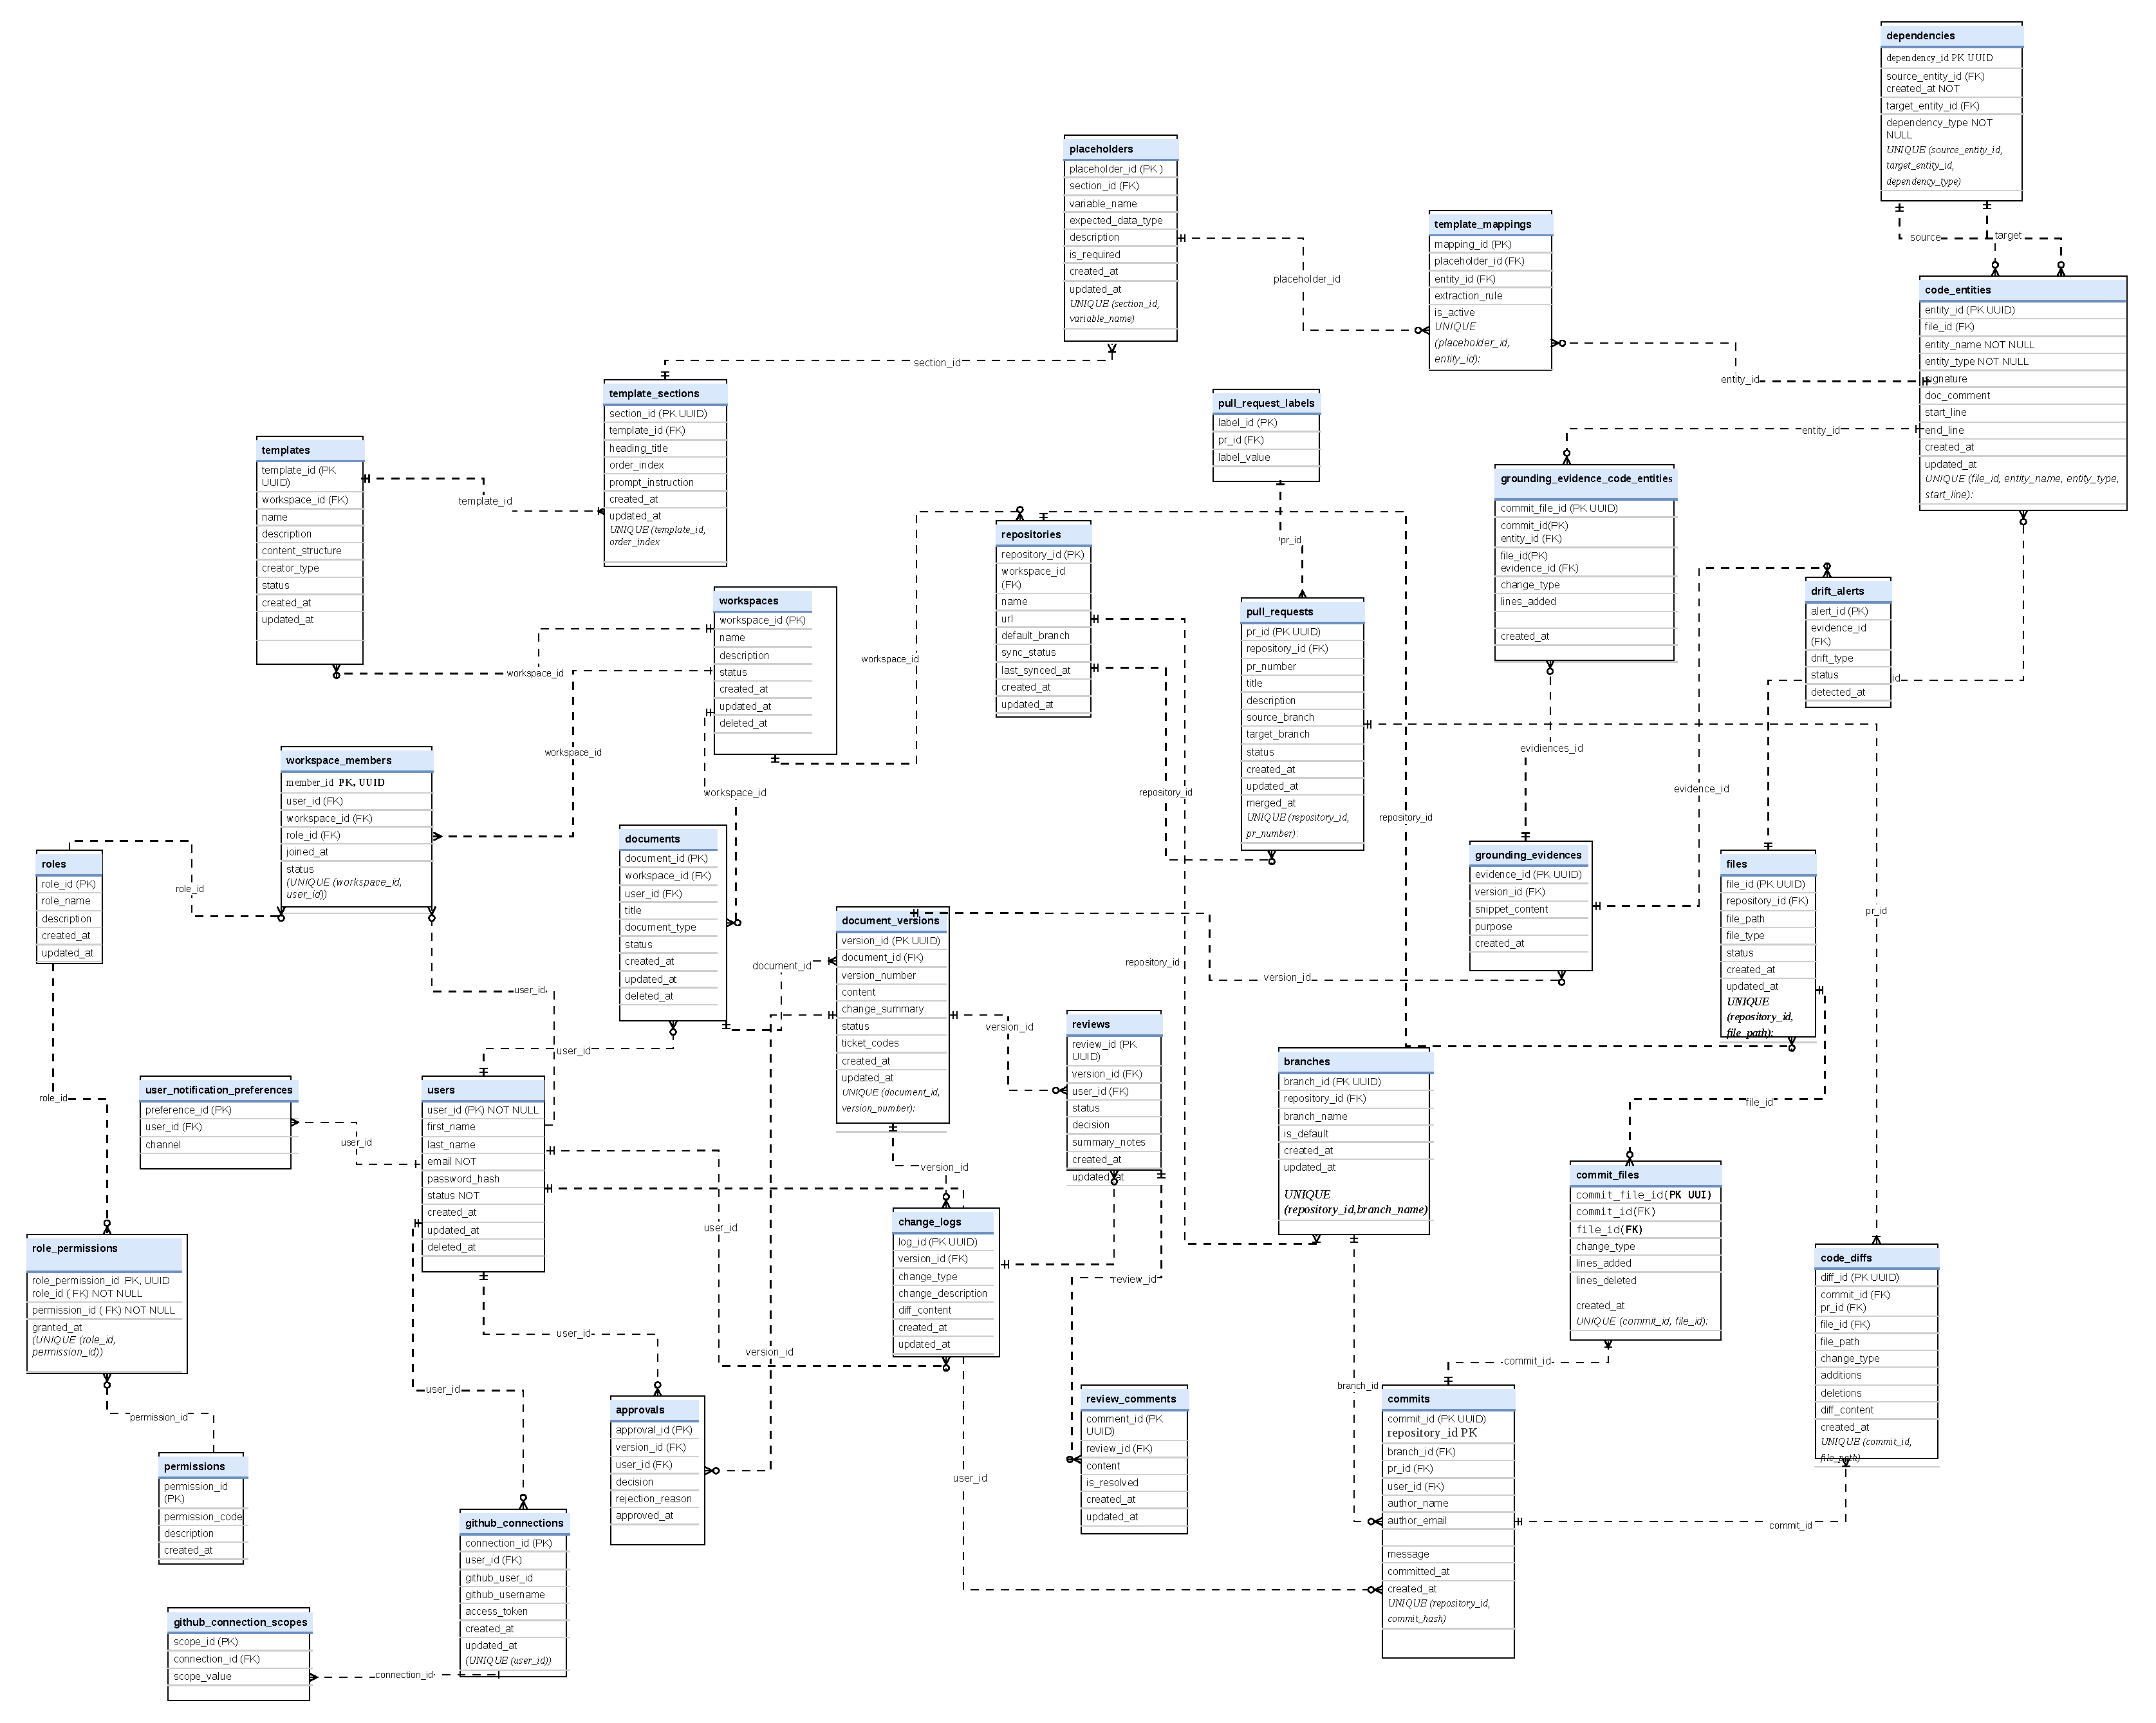
\includegraphics[
        width=\textwidth,
        height=0.75\textheight,
        keepaspectratio
    ]{./images/erd_muc_logic.pdf}
    \caption{Sơ đồ ERD mức logic}
    \label{fig:erd-logic}
\end{figure}



\chapter{Tổng kết Lược đồ Quan hệ Lô-gíc-Chuẩn hóa 3NF (Stage 2)}\label{c:erd_logic}

\section{Sơ đồ ERD mức logic}

\begin{figure}[H]
    \centering
    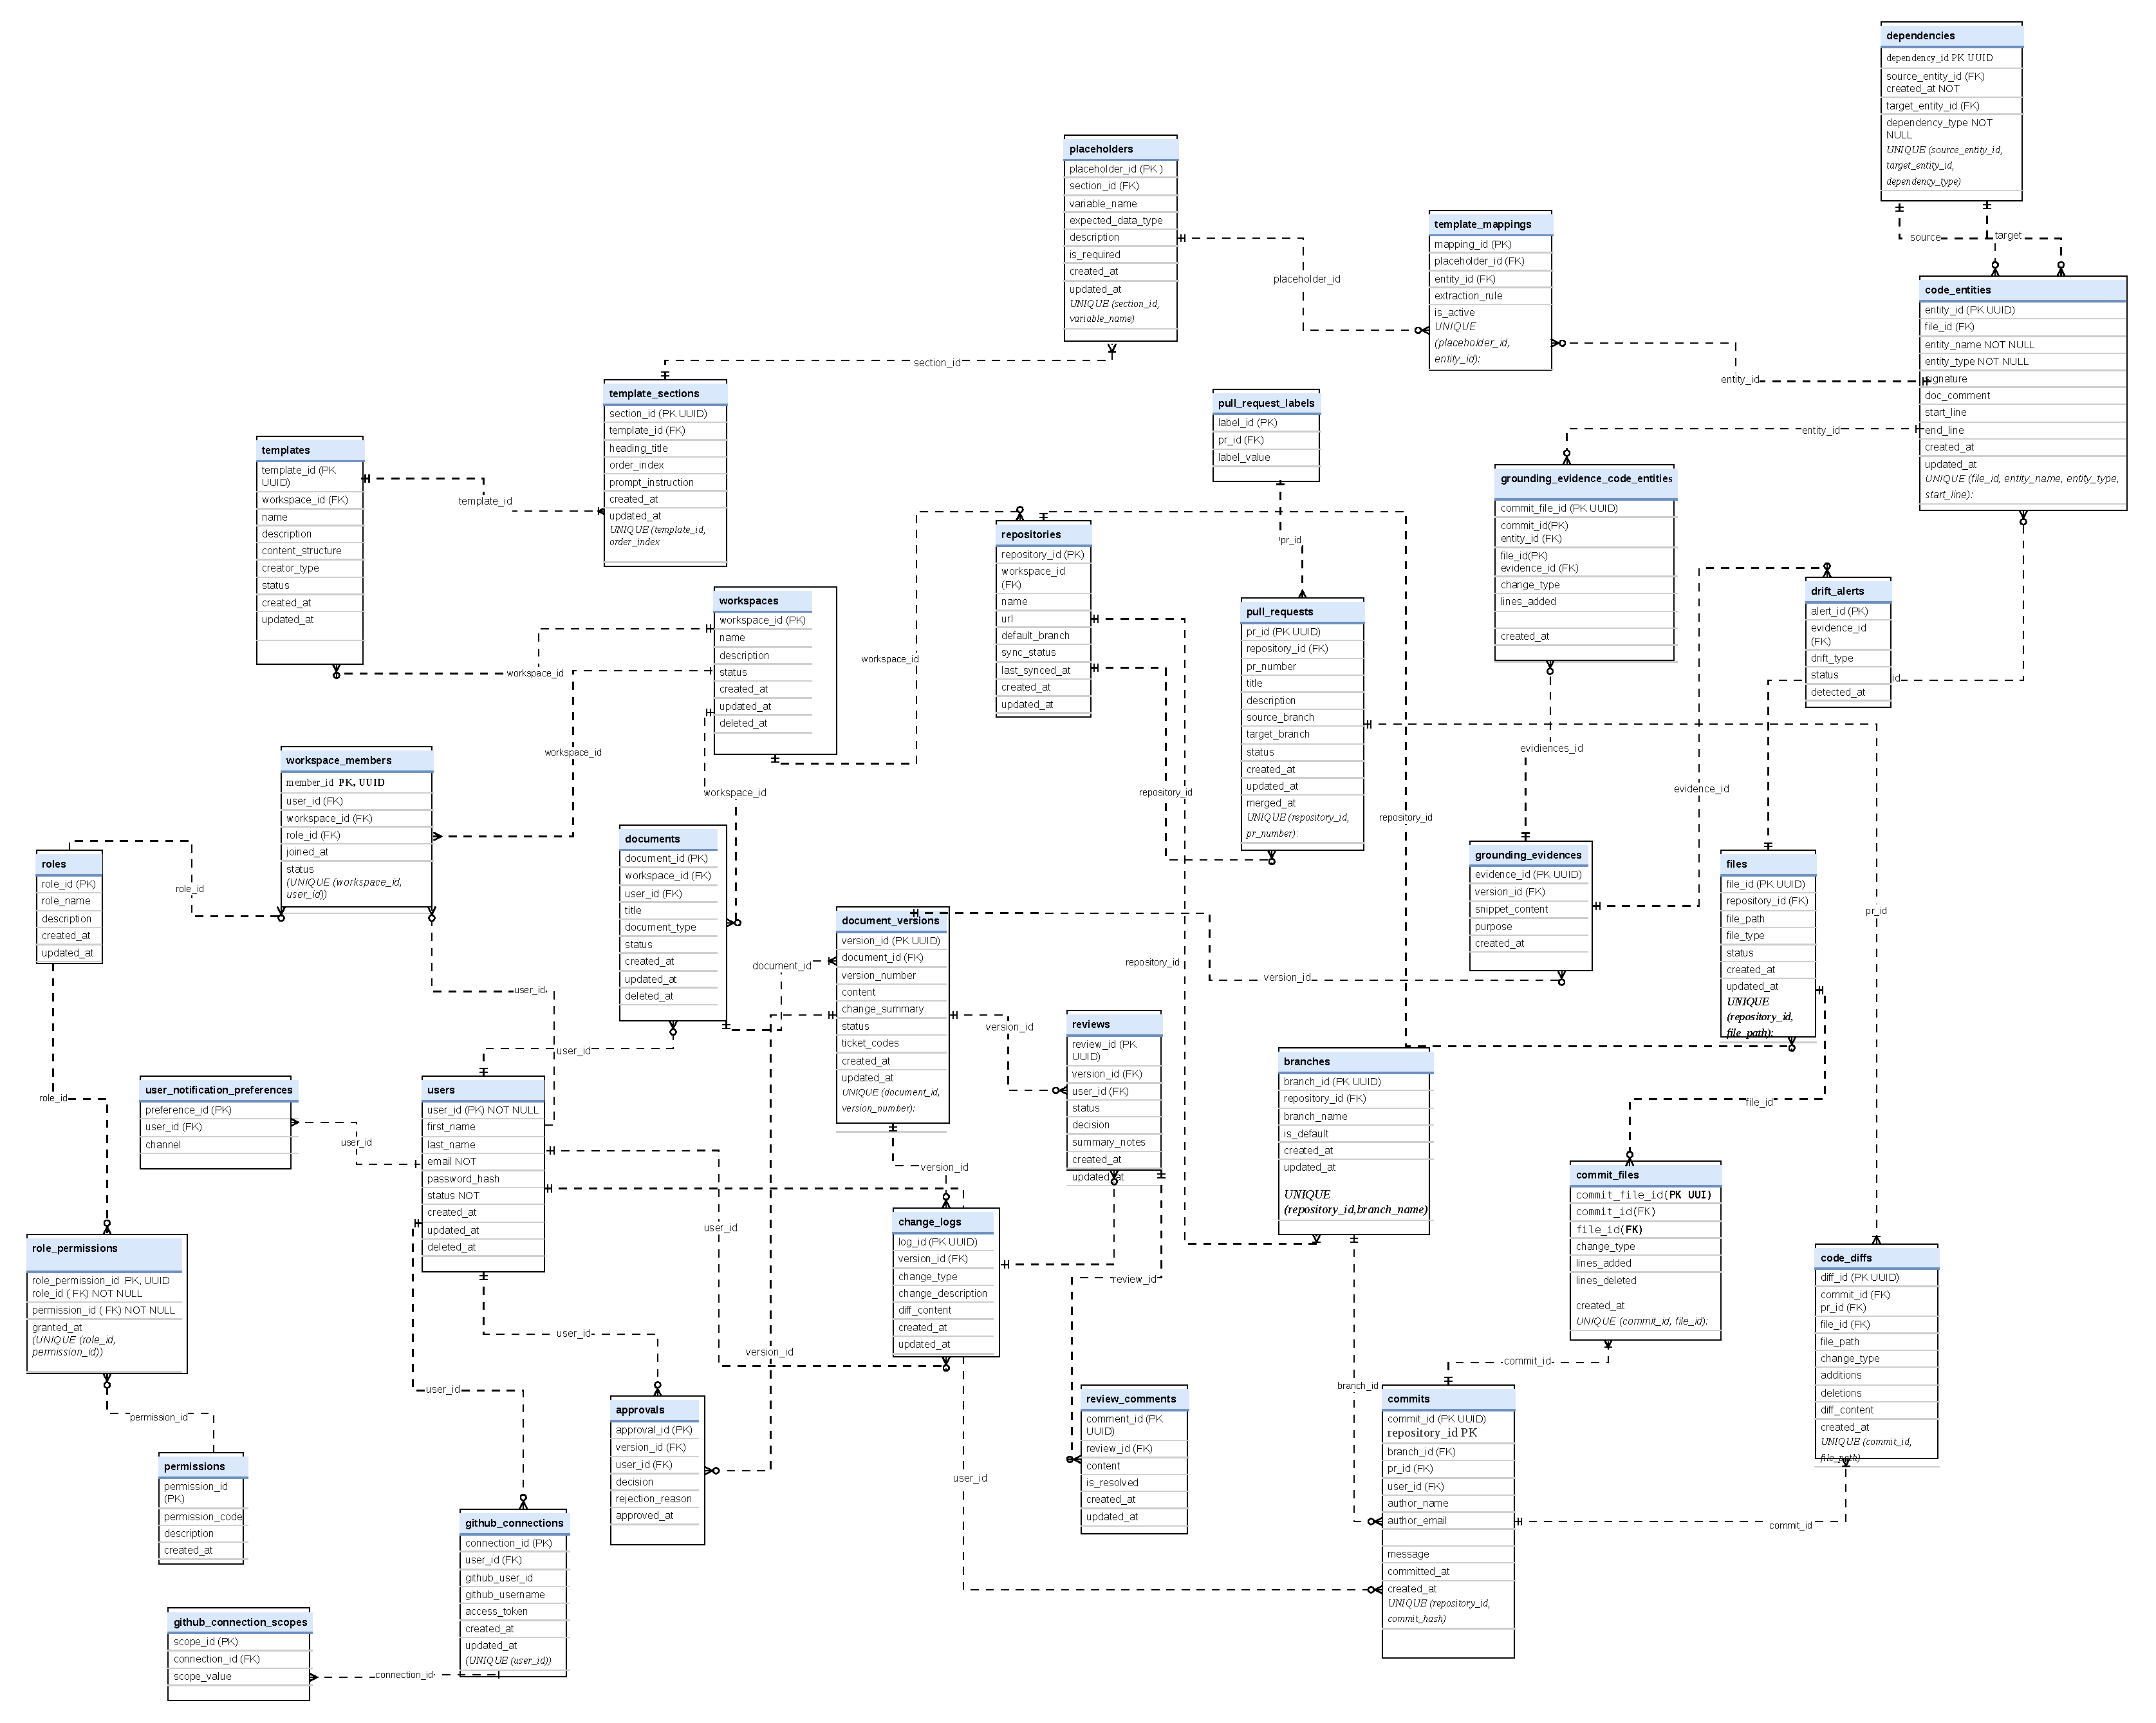
\includegraphics[
        width=\textwidth,
        height=0.75\textheight,
        keepaspectratio
    ]{./images/erd_muc_logic.pdf}
    \caption{Sơ đồ ERD mức logic}
    \label{fig:erd-logic}
\end{figure}
\chapter{Further results}\label{c:further}

Đề tài đã hoàn thành xuất sắc quy trình thiết kế cơ sở dữ liệu toàn diện cho hệ thống \textbf{LivingDocs} trải dài qua ba giai đoạn chuẩn hóa từ Stage 1 đến Stage 3. 
Ở Mức quan niệm (Stage 1), mô hình ERD và UML Class Diagram đã chuẩn hóa thành công các thực thể nghiệp vụ phức tạp như phân quyền Scoped RBAC, luồng kiểm duyệt 2 cấp và cơ chế lưu minh chứng AI. 
Chuyển sang Mức logic (Stage 2), hệ thống được ánh xạ chính xác sang Lược đồ quan hệ và chứng minh đạt chuẩn 3NF, giúp loại bỏ triệt để sự dư thừa dữ liệu cũng như các bất thường khi thêm, sửa, xóa. 
Tại Mức vật lý (Stage 3), các bảng được tối ưu hóa kiểu dữ liệu, hệ thống chỉ mục (Index) và ràng buộc toàn vẹn nhằm nâng cao hiệu năng truy vấn ở mức tối đa. 
Kết quả thu được tạo nên một nền tảng kiến trúc dữ liệu vững chắc, sẵn sàng đáp ứng khả năng mở rộng và vận hành ổn định cho dự án khi triển khai thực tế. 
Đây là minh chứng rõ nét cho tính hiệu quả của việc áp dụng quy trình thiết kế CSDL bài bản vào việc xây dựng một hệ thống phần mềm chuyên nghiệp.

\chapter{Extensions}\label{c:extensions}

This chapter sketches extensions of the framework. Temporibus autem quibusdam et aut officiis debitis aut rerum necessitatibus saepe eveniet, ut et voluptates repudiandae sint et molestiae non recusandae. Itaque earum rerum hic tenetur a sapiente delectus, ut aut reiciendis voluptatibus maiores alias consequatur aut perferendis doloribus asperiores repellat.

\section{First extension}\label{s:extensions}

The following list summarizes possible directions for future work:
\begin{enumerate}
\item Et harum quidem rerum facilis est et expedita distinctio.
\item Nam libero tempore, cum soluta nobis est eligendi optio.
\item Cumque nihil impedit, quo minus id, quod maxime placeat, facere possimus, omnis voluptas assumenda est.
\item Temporibus autem quibusdam et aut officiis debitis aut rerum necessitatibus saepe eveniet.
\end{enumerate}
Lorem ipsum dolor sit amet, consectetur adipiscing elit\index{elit}. Nulla facilisi. Nullam molestie, libero sit amet luctus vehicula, eros purus ultrices libero, eget fermentum leo sapien a metus. Duis porta massa vel justo posuere, nec placerat neque dictum. Morbi nec velit in turpis fermentum cursus nec ut leo. Integer vitae eros vehicula, fermentum turpis sed, fermentum elit.\footnote{Extensions are left for future work. Temporibus autem quibusdam et aut officiis debitis aut rerum necessitatibus saepe eveniet, ut et voluptates repudiandae sint et molestiae non recusandae. Itaque earum rerum hic tenetur a sapiente delectus.}

\section{Second extension}

One may also consider the following. Pellentesque habitant morbi tristique senectus et netus et malesuada fames ac turpis egestas. Aliquam erat volutpat. Donec tincidunt, quam sed pellentesque fermentum, lorem dolor consequat lectus, at pulvinar arcu ipsum in ligula. Mauris pretium ipsum id sapien posuere vehicula. Vivamus consectetur, turpis vitae pellentesque molestie, libero odio venenatis mauris, id vestibulum nisl nulla sit amet enim. See \citet{LMS18a,LMS18b} for related work.

Lorem ipsum dolor sit amet, consectetur adipiscing elit. Sed ullamcorper justo nec sem blandit, ac interdum libero convallis. Nulla facilisi. Etiam euismod, purus eget tempor feugiat, lectus ex vehicula justo, ut feugiat odio nisi sit amet lorem. Vivamus id lobortis justo. Sed varius scelerisque nibh, ut finibus quam vehicula nec. Cras ultricies consectetur ex, sit amet vestibulum lacus hendrerit vel. Sed lacinia eleifend purus. Nunc dignissim eros et sapien lacinia eleifend. Curabitur sit amet velit eu metus suscipit tempus. Maecenas in libero felis. Sed quis eros sapien. Suspendisse potenti.

\section{Third extension}

Curabitur maximus libero id magna bibendum fringilla. Curabitur ultricies dictum justo. Nam efficitur lobortis sapien a tristique. Vivamus vestibulum, sem nec dignissim scelerisque, purus nunc volutpat ligula, vitae aliquam libero orci nec augue. Nullam semper pulvinar turpis eget finibus. Suspendisse potenti. Nunc posuere arcu eget mauris venenatis, id pharetra sapien dapibus. Etiam at dictum urna. Integer gravida, odio sit amet mattis scelerisque, ipsum arcu ullamcorper sem, in vehicula sapien elit in tellus. Cras nec justo eu mauris volutpat dignissim. Curabitur malesuada purus sed tortor sollicitudin, in ullamcorper risus suscipit. Sed auctor tortor non libero suscipit, nec vehicula velit consequat. Integer nec est at lacus venenatis malesuada sed nec tortor. Sed aliquam urna non nunc luctus, eget cursus purus consequat. Vivamus a purus nec purus finibus ultricies. Suspendisse potenti.


\part{Conclusion}\label{p:conclusion}

\chapter{Summary}\label{c:summary}

% Summary chapter: enter main findings and takeaways from the book.

\section{Main findings} 

This book has presented a template for academic books. The initial chapters introduced the structure: an introduction, sections and subsections with references and paragraphs, and a chapter on mathematical typesetting. The next chapters illustrated lists, figures, and tables; cross-references and conclusion; further results; and extensions. Sed ut perspiciatis, unde omnis iste natus error sit voluptatem accusantium doloremque laudantium, totam rem aperiam eaque ipsa, quae ab illo inventore veritatis et quasi architecto beatae vitae dicta sunt, explicabo.

\section{Key takeaways} 

Nemo enim ipsam voluptatem, quia voluptas sit, aspernatur aut odit aut fugit, sed quia consequuntur magni dolores eos, qui ratione voluptatem sequi nesciunt, neque porro quisquam est, qui dolorem ipsum, quia dolor sit amet consectetur adipiscing velit, sed quia non numquam eius modi tempora incidunt, ut labore et dolore magnam aliquam quaerat voluptatem. At vero eos et accusamus et iusto odio dignissimos ducimus, qui blanditiis praesentium voluptatum deleniti atque corrupti, quos dolores et quas molestias excepturi sint, obcaecati cupiditate non provident, similique sunt in culpa, qui officia deserunt mollitia animi, id est laborum et dolorum fuga.

\section{Closing remark} 

Itaque earum rerum hic tenetur a sapiente delectus, ut aut reiciendis voluptatibus maiores alias consequatur aut perferendis doloribus asperiores repellat. Lorem ipsum dolor sit amet, consectetur adipiscing elit\index{elit}. Sed do eiusmod\index{eiusmod} tempor incididunt ut labore et dolore magna aliqua. Ut enim ad minim veniam, quis nostrud exercitation ullamco laboris nisi ut aliquip ex ea commodo consequat. Duis aute irure dolor in reprehenderit in voluptate velit esse cillum dolore eu fugiat nulla pariatur. Excepteur sint occaecat cupidatat non proident, sunt in culpa qui officia deserunt mollit anim id est laborum.


\chapter{Future research}\label{c:future}

% Future research chapter: enter open questions and directions.

\section{Open questions}

Several directions remain for future work. First, one could extend the framework to allow for such-and-such. Second, it would be valuable to incorporate this-and-that and to relax certains assumptions. Third, empirical applications to such-and-such domain would help assess the quantitative relevance of the results. Lorem ipsum dolor sit amet, consectetur adipiscing elit. Sed do eiusmod tempor\index{tempor} incididunt ut labore et dolore magna aliqua. Ut enim ad minim veniam, quis nostrud exercitation ullamco laboris nisi ut aliquip ex ea commodo consequat.

\section{Related literature}

Duis aute irure dolor in reprehenderit in voluptate velit esse cillum dolore eu fugiat nulla pariatur. Excepteur sint occaecat cupidatat non proident, sunt in culpa qui officia deserunt mollit anim id est laborum. Pellentesque habitant morbi tristique senectus et netus et malesuada fames ac turpis egestas. Aliquam erat volutpat. Donec tincidunt, quam sed pellentesque fermentum, lorem dolor consequat lectus, at pulvinar arcu ipsum in ligula.

\section{Concluding remarks}

Mauris pretium ipsum id sapien posuere vehicula. Vivamus consectetur, turpis vitae pellentesque molestie, libero odio venenatis mauris, id vestibulum nisl nulla sit amet enim. Integer vitae metus eget risus vulputate consectetur. Suspendisse potenti. Quisque dictum purus non justo aliquet, sed tristique odio dapibus. Sed tincidunt justo vitae leo mattis, a ullamcorper metus vestibulum. Sed ac sapien metus. Sed non mauris nec nisl vehicula iaculis eget eget enim. Suspendisse potenti. Sed ac purus volutpat, venenatis sem eget, fermentum lorem. Suspendisse eu convallis tortor. Nunc vel dictum libero. Cras eleifend, orci non faucibus gravida, sapien quam pharetra ligula, nec tincidunt elit ex at sapien.


\appendix

\part{Technical appendix}\label{p:appendix}

\chapter{Generic technical topic}\label{a:appendix1}

This is a generic appendix. Obcaecati cupiditate non provident, similique sunt in culpa, qui officia deserunt mollitia animi, id est laborum\index{laborum} et dolorum fuga. Duis aute irure dolor in reprehenderit in voluptate\index{voluptate} velit esse cillum dolore eu fugiat nulla pariatur. Excepteur sint occaecat cupidatat non proident, sunt in culpa qui officia deserunt mollit anim id est laborum. 

\section{Generic appendix section} 

This is a generic subsection in the appendix. Lorem ipsum dolor sit amet, consectetur adipisicing elit, sed do eiusmod tempor incididunt ut labore et dolore magna aliqua. Ut enim ad minim veniam, quis nostrud exercitation ullamco laboris nisi ut aliquip ex ea commodo consequat\index{consequat}. 

In efficitur mi sed eros tincidunt tempus. Cras ut neque vehicula, convallis odio in, lacinia orci. Vivamus et nunc vestibulum, efficitur eros vitae, bibendum justo. Aenean tincidunt ligula ut augue pulvinar, ut placerat risus accumsan. Integer pellentesque odio ac commodo dictum. Ut ut justo a mi consequat vestibulum. 

Lorem ipsum dolor sit amet, consectetur adipiscing elit. Fusce gravida aliquam velit, sed fermentum\index{fermentum} odio fermentum eu. Donec eget fermentum ligula. Nulla facilisi. Integer vitae metus eget risus vulputate consectetur. Suspendisse potenti. Quisque dictum purus non justo aliquet, sed tristique odio dapibus. Sed tincidunt justo vitae leo mattis, a ullamcorper metus vestibulum. Sed ac sapien metus. Sed non mauris nec nisl vehicula iaculis eget eget enim. Suspendisse potenti. Sed ac purus volutpat, venenatis sem eget, fermentum lorem. Suspendisse eu convallis tortor. Suspendisse potenti. Nunc vel dictum libero. Cras eleifend, orci non faucibus gravida, sapien quam pharetra ligula, nec tincidunt elit ex at sapien. 

\section{Assumptions and theorems and proofs}

This section displays an assumption and results to illustrate how they are typeset and numbered in the appendix. Note in particular that numbering of all the results is specific to each appendix (just as it is specific to each chapter in the main matter). First is an assumption:
\begin{assumption} 
Similique sunt in culpa, qui officia deserunt mollitia animi, id est laborum et dolorum fuga:
\begin{equation*}
\mathbb{E}(\Omega_{m,n}) = \mathbb{P}(\omega\cdot \mu - \xi) - \sum_{i=0}^{m}\sum_{j=1}^{n} \sigma(i,j) + 123^{56}.
\end{equation*}
Curabitur volutpat ultrices nunc id efficitur. Donec posuere, dui vel gravida elementum, ligula nisi lobortis elit, eu aliquet quam ligula id libero. Sed ac efficitur tur.
\label{a:appe}\end{assumption}

Lorem ipsum dolor sit amet, consectetur adipisicing elit, sed do eiusmod
tempor incididunt ut labore et dolore magna aliqua. Ut enim ad minim veniam,
quis nostrud exercitation ullamco laboris nisi ut aliquip ex ea commodo
consequat. Next is a theorem---numbering is specific to each type of entry, so theorems have a separate numbering from assumptions:
\begin{theorem}
Duis aute irure dolor in reprehenderit in voluptate velit esse
cillum dolore eu fugiat nulla pariatur. Excepteur sint occaecat cupidatat non
proident, sunt in culpa qui officia deserunt mollit anim id est laborum:
\begin{equation}
X^* =\iint_{0}^{\infty} \alpha(i) \cdot \mathcal{A}^2(i) + \mathbb{P}(X\mid Z(i))\,di\,dj,\end{equation}
integer vestibulum sapien nec velit varius, nec scelerisque nunc eleifend. Cras sollicitudin, justo sit amet tempus vehicula, ex ex vulputate nulla, non vestibulum quam tortor nec nisl. 
\end{theorem}

Lorem ipsum dolor sit amet, consectetur adipiscing elit. Sed aliquam magna vel urna ultrices, sed lacinia nulla mattis. Fusce non nunc nec est mollis malesuada. Here is another theorem---continuing the numbering:
\begin{theorem}
Consectetur adipiscing elit, sed do eiusmod tempor incididunt ut labore et dolore magna aliqua: $y(\gamma) \geq 3\pi + \cos(\vartheta)$.
\label{t:theorem1}\end{theorem}

\begin{proof}
Based on assumption~\ref{a:appe}, lorem ipsum dolor sit amet, consectetur adipiscing elit. Sed aliquam magna vel urna ultrices, sed lacinia nulla mattis. Fusce non nunc nec est mollis malesuada. Nullam dignissim nulla sit amet libero facilisis, eget fringilla libero sagittis. Suspendisse potenti. Vivamus fermentum consectetur ante, at rhoncus nisi tristique vel. Vivamus in est quis justo fermentum lacinia ac eu leo. Maecenas nec tempor nisi---as in theorem \ref{t:theorem1}.
\end{proof}

\section{More math}

Here is math and equations in the appendix---see equations \eqref{e:appendix1} and \eqref{e:experiments}. Temporibus autem quibusdam $\xi$ et aut officiis debitis aut rerum necessitatibus saepe eveniet ut et voluptates repudiandae sint et molestiae non recusandae $1-\gamma$. Itaque earum rerum hic $\mathcal{S}(\zeta^0)$ tenetur a sapiente delectus $\mathcal{B}^\theta$, ut aut reiciendis voluptatibus maiores alias consequatur aut perferendis doloribus asperiores repellat $\mathbb{V}^i$:
\begin{equation}
\mathbb{V}^r = (1-\gamma) \times 0 +\gamma S(z^*) v^s+\gamma [1-S(z^*)] \mathcal{V}^i-c.
\label{e:appendix1}\end{equation}

Ut enim ad minima veniam, quis nostrum exercitationem ullam corporis suscipit laboriosam, nisi ut aliquid ex ea commodi consequatur? Quis autem vel eum iure reprehenderit qui in ea voluptate velit esse quam nihil molestiae consequatur, vel illum qui dolorem eum fugiat quo voluptas nulla pariatur? 
\begin{equation}
\mathbb{E}(N(z)) = \frac{1}{1-\gamma F(z)}.
\label{e:experiments}\end{equation}


\chapter{Another technical topic}\label{a:appendix2}

Here is a second appendix. At vero eos et accusamus et iusto odio dignissimos ducimus, qui blanditiis praesentium voluptatum\index{voluptatum} deleniti atque corrupti.

\section{Larger figure, without panel, in the appendix} 

Here is a large, simple figure in the appendix---illustrating how figures are set and numbered in the appendix (see figure \ref{f:appendix1}). At vero eos et accusamus et iusto odio dignissimos ducimus, qui blanditiis praesentium voluptatum deleniti atque corrupti, quos dolores et quas molestias excepturi sint, obcaecati cupiditate non provident, similique sunt in culpa, qui officia deserunt mollitia animi, id est laborum et dolorum fuga.\footnote{The numbering of the footnotes restarts at the beginning of each chapter and appendix. Nemo enim ipsam voluptatem quia voluptas sit aspernatur aut odit aut fugit, sed quia consequuntur magni dolores eos qui ratione voluptatem sequi nesciunt---sed quia consequuntur magni dolores eos qui ratione voluptatem sequi nesciunt.} Duis aute irure dolor in reprehenderit in voluptate velit esse
cillum dolore eu fugiat nulla pariatur. Excepteur sint occaecat cupidatat non
proident, sunt in culpa qui officia deserunt mollit anim id est laborum.

\begin{figure}[t]
\includegraphics[scale=0.3,page=1]{\pdf}
\caption{Single figure in the appendix}
\note[Note]{This is the note for the larger graph. Nam libero tempore, cum soluta nobis est eligendi optio, cumque nihil impedit, quo minus id, quod maxime placeat, facere possimus---cumque nihil impedit, quo minus id, quod maxime placeat, facere possimus.}
\note[Source]{Figure borrowed from a paper by \citet{MM26}.}
\label{f:appendix1}\end{figure}

Lorem ipsum dolor sit amet, consectetur adipisicing elit, sed do eiusmod
tempor incididunt ut labore et dolore magna aliqua. Ut enim ad minim veniam,
quis nostrud exercitation ullamco laboris nisi ut aliquip ex ea commodo
consequat. Duis aute irure dolor in reprehenderit in voluptate velit esse
cillum dolore eu fugiat nulla pariatur. Excepteur sint occaecat cupidatat non
proident, sunt in culpa qui officia deserunt mollit anim id est laborum.

Nullam fringilla, risus sit amet tincidunt sagittis, ligula nisi suscipit nisi, nec vulputate libero odio sit amet metus. Sed auctor elit nec orci venenatis, in dignissim lacus venenatis. Curabitur auctor odio sit amet leo molestie, vel lacinia sem congue. Integer id interdum metus. Ut ultrices ultricies lorem eget egestas. Integer efficitur libero id sapien posuere, at laoreet mauris consectetur. Nulla facilisi. Sed dapibus lectus at lacus interdum, ac vehicula dui bibendum. In hac habitasse platea dictumst. Sed luctus metus quis libero ultrices, vitae fringilla purus varius. Sed efficitur suscipit felis vel dapibus. Nunc condimentum laoreet ipsum, ut faucibus risus sodales sed. Sed dignissim, magna vel suscipit fermentum, lectus lorem suscipit tortor, eu suscipit elit tortor non dolor. 

\section{A foonote}

Here is a sentence with a footnote.\footnote{Nemo enim ipsam voluptatem quia voluptas sit aspernatur aut odit aut fugit, sed quia consequuntur magni dolores eos qui ratione voluptatem sequi nesciunt. Duis aute irure dolor in reprehenderit in voluptate velit esse
cillum dolore eu fugiat nulla pariatur. Excepteur sint occaecat cupidatat non
proident, sunt in culpa qui officia deserunt mollit anim id est laborum.}

Lorem ipsum dolor sit amet, consectetur adipisicing elit, sed do eiusmod tempor incididunt ut labore et dolore magna aliqua. Ut enim ad minim veniam,
quis nostrud exercitation ullamco laboris nisi ut aliquip ex ea commodo
consequat.\footnote{Nemo enim ipsam voluptatem quia voluptas sit aspernatur aut odit aut fugit, sed quia consequuntur magni dolores eos qui ratione voluptatem sequi nesciunt.}

\section{References}\label{a:subappendix}

Here is a sentence with some references in text: \citet{MS19,MS21} found something but that is an uncommon result. The references can also go in parentheses at the end of the sentence \citep{MS21,MS22}. The references go to the reference list at the end of the book---so appendix and main text share a common reference list.

Lorem ipsum dolor sit amet, consectetur adipisicing elit, sed do eiusmod
tempor incididunt ut labore et dolore magna aliqua. Ut enim ad minim veniam,
quis nostrud exercitation ullamco laboris nisi ut aliquip ex ea commodo
consequat.


\chapter{Last technical topic}\label{a:appendix3}

This is a last appendix with a bit of text.

\section{A first section}

Sed vestibulum\index{vestibulum} ex a tristique lacinia. Integer interdum magna vel magna rutrum fermentum. Maecenas sed mi in nunc convallis rutrum. Vivamus dapibus bibendum est, ac tincidunt ipsum fermentum id. Nunc id est turpis. Suspendisse potenti. Sed ac laoreet nulla, eu sollicitudin libero. Suspendisse tempus orci nec mauris volutpat eleifend. Integer nec tristique libero. Sed vehicula ipsum sit amet magna accumsan, nec pulvinar nisl consequat. In ac hendrerit turpis. Sed aliquet luctus mauris, vitae congue turpis. Nullam blandit lacus vel interdum eleifend. 

\section{A second section}

Nam pretium mauris eros, nec sollicitudin risus tincidunt a. Vivamus in augue vitae ligula scelerisque dapibus. Integer eget metus aliquet, efficitur nibh eget, pharetra eros. Suspendisse luctus interdum ex id suscipit. Donec quis augue mauris. Nulla ut erat eget nisl hendrerit malesuada. Vivamus eu tortor sit amet sem fringilla eleifend. In hac habitasse platea dictumst. Suspendisse potenti. Ut eget libero sed orci tempor ullamcorper:
\begin{equation}
S^*(z) = \frac{\alpha}{1-\gamma (1-\alpha)} > \int\frac{\alpha(i)}{\gamma(i)}\,di.
\label{e:type1Classical}\end{equation}

Nam pretium mauris eros, nec sollicitudin risus tincidunt a. Vivamus in augue vitae ligula scelerisque dapibus. Integer eget metus aliquet, efficitur nibh eget, pharetra eros. Suspendisse luctus interdum ex id suscipit. Donec quis augue mauris. Nulla ut erat eget nisl hendrerit malesuada. Vivamus eu tortor sit amet sem fringilla eleifend. In hac habitasse platea dictumst. Suspendisse potenti. Ut eget libero sed orci tempor ullamcorper:
\begin{align}
\mathcal{W}^{2}(\zeta) &= \left[\frac{\beta}{1-\nu (1-\xi)}\right] \pm \Lambda\\
\mathcal{L}^{2}(\zeta) &= \left(\frac{\beta}{1-\nu (1-\xi)}\right) \\
\overline{a-b} &= \int_0^{+\infty} \frac{\beta}{1-\nu(x) (1-\xi)}\,dx \in \mathbb{R}.
\end{align}


\section{A third section}

Lorem ipsum dolor sit amet, consectetur adipiscing elit. Sed aliquam magna vel urna ultrices, sed lacinia nulla mattis. Fusce non nunc nec est mollis malesuada. Nullam dignissim nulla sit amet libero facilisis, eget fringilla libero sagittis. Suspendisse potenti. Vivamus fermentum consectetur ante, at rhoncus nisi tristique vel. Vivamus in est quis justo fermentum lacinia ac eu leo. Sed ac pulvinar nulla. Etiam quis felis dapibus, vulputate metus eu, finibus nunc. Sed vel sodales dui. Nam venenatis dolor non orci tempus fermentum. Vivamus sodales justo a ligula cursus aliquet. Sed fringilla nunc vitae justo finibus, id placerat lectus sodales.


\backmatter

\bibliography{\bib}

\chapter{Acknowledgments}

% Enter acknowledgment text:

Many friends and colleagues, by their advice and criticism, have helped to shape this book. I thank in particular so-and-so for such-and-such. I am grateful to such-and-such institution for financial support. I thank my editor and the reviewers for their helpful comments.

Nemo enim ipsam voluptatem, quia voluptas sit, aspernatur aut odit aut fugit, sed quia consequuntur magni dolores eos, qui ratione voluptatem sequi nesciunt, neque porro quisquam est, qui dolorem ipsum, quia dolor sit amet consectetur adipiscing velit, sed quia non numquam eius modi tempora incidunt, ut labore et dolore magnam aliquam quaerat voluptatem. At vero eos et accusamus et iusto odio dignissimos ducimus, qui blanditiis praesentium voluptatum deleniti atque corrupti, quos dolores et quas molestias excepturi sint, obcaecati cupiditate non provident, similique sunt in culpa, qui officia deserunt mollitia animi, id est laborum et dolorum fuga.

\printindex

\end{document}